\documentclass{article}

% ready for submission
\usepackage[final]{neurips_2024} % Use 'final' option to display authors

\usepackage[utf8]{inputenc} % allow utf-8 input
\usepackage[T1]{fontenc}    % use 8-bit T1 fonts
\usepackage{hyperref}       % hyperlinks
\usepackage{url}            % simple URL typesetting
\usepackage{booktabs}       % professional-quality tables
\usepackage{amsfonts}       % blackboard math symbols
\usepackage{nicefrac}       % compact symbols for 1/2, etc.
\usepackage{microtype}      % microtypography
\usepackage{xcolor}         % colors
\usepackage{graphicx}
\usepackage{subcaption} % Add this in the preamble
\usepackage{float}
\usepackage{multirow}
\bibliographystyle{unsrt}

\title{Optimizing Graph Neural Networks for Enhanced Community Detection in Social Networks
}

\author{%
  Parsa Kamalipour\\
  Department of Computer Science \\
  Concordia University \\
  \texttt{parsa.kamalipour@mail.concordia.ca} 
  \And
  Abdulmoumen Al-Atrash \\
  Department of Computer Science \\
  Concordia University \\
  \texttt{a\_alatr@live.concordia.ca} 
  \And
  Aniket Roy \\
  Department of Computer Science \\
  Concordia University \\
  \texttt{aniket.roy@mail.concordia.ca} 
}

\begin{document}

\maketitle

\begin{abstract}
% This abstract provides a concise overview of the project proposal, including the problem being addressed, motivation, and approach. Keep it brief, within one paragraph.
% Community detection, which is a main problem in social network analysis, looks to find clusters in graphs where nodes are more connected with each other than with the rest of the network. This is important in different fields like social network analysis and biology, and it helps in understanding complex systems and their organization. Moreover, the recent growth of social networks through the inherent interconnectedness of the internet has made properly analyzing these intricate structures increasingly important. Traditional methods like modularity optimization and spectral clustering have limitations in handling large networks and often miss detailed community structures. Optimization-based approaches, like Learning-Based Genetic Algorithms (LGA) and Quantum-Inspired Optimization, achieve impressive accuracy but struggle with generalizing to networks of varying complexity and domains. Similarly, modularity-based methods, while interpretable and computationally efficient, rely too heavily on modularity maximization and can fail to distinguish between communities within networks of varying sizes, limiting their effectiveness. Deep learning excels at capturing complex relationships but can be computationally intensive when applied to large-scale networks. One notable model, Graph Neural Networks (GNNs), has emerged as a powerful deep learning approach to solving the community detection problem. GNNs have demonstrated significant potential in overcoming the challenges faced by traditional methods, including issues with scalability, accuracy, and adaptability to networks of diverse sizes and complexities. This project aims to solve these limitations by using machine learning, specifically GNNs, due to their strong capabilities of identifying key patterns in complex data networks by effectively learning the high-dimensional feature representations of nodes and communities. With these tools, the project tries to make community detection more accurate and scalable. This plan aligns with course objectives, where we apply theoretical knowledge to practical problems in network analysis and machine learning. It addresses gaps in the existing methodologies for solving community detection by highlighting the merit of GNNs over traditional methods. Additionally, scalable enhancements such as graph sampling methods, optimized graph convolutions, and graph partitioning strategies are investigated to address the computational challenges associated with large-scale networks.
Community detection, a key problem in social network analysis, identifies clusters in graphs where nodes are more interconnected than with the rest of the network. This has applications in fields like social network analysis and biology, aiding in understanding complex systems. The rapid growth of social networks has made analyzing these intricate structures increasingly critical. Traditional methods, such as modularity optimization and spectral clustering, struggle with large networks and often miss finer community structures. Optimization-based approaches like Learning-Based Genetic Algorithms (LGA) and Quantum-Inspired Optimization show high accuracy but lack generalization across diverse networks. Modularity-based methods, while efficient, rely heavily on modularity maximization, limiting their effectiveness in distinguishing communities in networks of varying sizes. Deep learning, particularly Graph Neural Networks (GNNs), has proven effective in addressing these challenges, offering scalability, accuracy, and adaptability to diverse networks. This project leverages GNNs to overcome these limitations by learning high-dimensional feature representations of nodes and communities, improving the accuracy and scalability of community detection. It aligns with course objectives by applying theoretical knowledge to practical problems in network analysis and machine learning, addressing gaps in traditional methods with enhancements like graph sampling, optimized graph convolutions, and graph partitioning.
\end{abstract}

\section{Introduction}
\subsection{Introduction to Community Detection}
% Describe the specific problem you aim to address in this project.
Community detection is all about identifying clusters or groups within a network - which are called communities - where nodes are more densely connected to each other than to the rest of the network. This problem is very crucial in various domains, including social network analysis, biology, and information retrieval, as it helps uncover the underlying structure and functional organization of complex systems. For instance, community detections in biology aid in identifying interconnected gene networks, while in social networks, they reveal social group dynamics and interaction patterns. Traditional methods, such as modularity optimization and spectral clustering, have been widely used for this purpose. However, these approaches often face challenges in handling large-scale networks and capturing intricate community structures, particularly when networks exhibit complex relationships or irregular structural patterns. As social networks continue to grow and become more deeply integrated into daily life, it is becoming vital to analyze these complex structures efficiently and on a large scale. This development demands advanced solutions that maintain performance while achieving scalability to keep up with the diverse and dynamic nature of real-world networks.

\subsection{Machine Learning Context}
% Outline the context within machine learning.
% Recent advancements and novelties in machine learning, particularly deep learning, have introduced lots of new methodologies for community detection. Graph Neural Networks (GNNs) have emerged as very powerful tools capable of learning complex patterns in graph-structured data. For instance, the Contrastive Deep Nonnegative Matrix Factorization (CDNMF) model integrates contrastive learning with deep nonnegative matrix factorization to enhance and improve on community detection by capturing both network topology and node attributes at the same time~\cite{li2024contrastivedeepnonnegativematrix}. Additionally, the integration of community detection algorithms with GNNs has been shown to improve link prediction tasks in scientific literature networks, demonstrating the synergistic potential of combining these approaches~\cite{liu2024communitydetectiongraphneural}. This highlights the latent potential of GNNs in addressing the limitations of modularity-based and optimization-based methods later discussed in this paper in offering both accuracy and scalability for complex networks.
Recent advancements in machine learning, particularly deep learning, have introduced numerous methodologies for community detection. Graph Neural Networks (GNNs) have proven to be powerful tools for learning complex patterns in graph-structured data. For example, the Contrastive Deep Nonnegative Matrix Factorization (CDNMF) model combines contrastive learning with deep nonnegative matrix factorization, capturing both network topology and node attributes to enhance community detection~\cite{li2024contrastivedeepnonnegativematrix}. Similarly, integrating community detection algorithms with GNNs has improved link prediction in scientific literature networks, showcasing the synergy of these approaches~\cite{liu2024communitydetectiongraphneural}. This underscores the potential of GNNs to overcome the limitations of modularity-based and optimization-based methods, offering greater accuracy and scalability for complex networks.

\subsection{Usage of Machine Learning in Community Detection}
% clearly define the aspects of the problem relevant to this course.
In this project, we aim to use machine learning techniques to address the challenges of community detection in large-scale networks, to be more precise in Social Networks. By using models such as GNNs and incorporating methods like optimization on previous ideas, we seek to develop an algorithm that can effectively identify communities with high accuracy and scalability. This approach aligns with the course objectives by applying machine learning methodologies to solve complex problems; thereby, by doing this research, we both learn a new Machine Learning methodology and also enhance our understanding of community structures in various real-world applications.

\subsection{Challenges in Community Detection}
% Traditional approaches to community detection face significant limitations that complicate their effectiveness in modern, large-scale applications. One major challenge for community detection when seeking to maintain high performance and robust detection capabilities is scalability~\cite{7161493}. In the real-world applications, networks are generated at massive scale and necessitate efficient processing, often demanding methods that can process millions or even billions of nodes and edges efficiently. Another complication lies in the inherently noisy and irregular nature of data within networks~\cite{10.1145/2488388.2488483}. Particularly, incorrect links, classified as false positives, and missing links, classified as false negatives, can distort community structures and lead to loss of accuracy for less nuanced methods. Finally, some networks tend to be heterogeneous such that nodes and edges can carry varying types of data~\cite{7536145}. This can pose issues to algorithms that rely heavily on structural relationships in the network to capture contextual information. Community detection is an inherently indeterminate problem---meaning that there is often no singular correct solution. This ambiguous nature demands robust methods that can generalize well to networks of diverse structures and sizes, which lays the foundation for the challenges explored in this paper.
Traditional approaches to community detection face notable limitations, particularly in modern large-scale applications. Scalability is a key challenge, as real-world networks often contain millions or billions of nodes and edges, requiring methods capable of efficient processing~\cite{7161493}. Another issue is the noisy and irregular nature of network data~\cite{10.1145/2488388.2488483}. False positives (incorrect links) and false negatives (missing links) can distort community structures, reducing accuracy for less sophisticated methods. Additionally, heterogeneous networks, where nodes and edges carry varying data types, pose challenges for algorithms reliant on structural relationships to capture context~\cite{7536145}. Community detection is inherently indeterminate, often lacking a single correct solution, demanding robust methods that generalize across diverse network structures and sizes. These challenges form the foundation for the discussions in this paper.

\section{Related Work}
\subsection{Overview}
This section presents a literature review to examine pre-existing knowledge in the area of the NP-Hard problem of 'Community Detection' in social networks. We examine relevant existing work to ensure that our proposed approach is justified based on the problem context and that it differs from already proposed solutions to the NP-Hard problem. In this section, we identify and discuss three main categories of algorithms used to tackle the problem of community detection, namely optimization-based methods, modularity-based approaches, and deep learning techniques.

\subsection{Optimization-Based Methods}
% A rather popular approach to solving challenging and inherently complex machine learning problems such as community detection is optimization. The Learning-Based Genetic Algorithm (LGA)~\cite{ABDI2024103031} [Identifying Communities in Complex Networks Using Learning-Based Genetic Algorithm] is designed to tackle the NP-hard nature of community detection problems. This method carefully combines Learning Automata with genetic operations to get around problems that genetic algorithms often have, such as unwanted premature convergence and local optima. The LGA achieves a notable improvement in accuracy of 26.47\% on real-world networks and a 48.32\% improvement on synthetic networks. Akbar et al.~\cite{Akbar2021} propose a quantum mechanics-inspired optimization approach that aims to detect underlying complex patterns, specifically in ecological communities. This paper simulates quantum principles for optimization detections for identifying patterns in biodiversity changes due to environmental factors such as land use and climate change. MARLCD~\cite{Alipour} is a multi-agent reinforcement learning algorithm designed for community detection within complex networks. The algorithm employs “agents” to independently explore communities within the network, updating actions on successful detections. MARLCD outperforms state-of-the-art methods such as GA-Net and Meme-Net when tested on both real and synthetic datasets. However, these three approaches lack generalizability on networks of varying domains and complexity, as their underlying assumptions make them effective within their respective applications but restrict their flexibility and may be computationally excessive when applied to networks with different structural patterns and complexities.
Optimization is a popular approach for tackling complex machine learning problems like community detection. The Learning-Based Genetic Algorithm (LGA)\cite{ABDI2024103031} [Identifying Communities in Complex Networks Using Learning-Based Genetic Algorithm] addresses the NP-hard nature of community detection by combining Learning Automata with genetic operations, overcoming issues like premature convergence and local optima. LGA achieves a 26.47\% accuracy improvement on real-world networks and a 48.32\% improvement on synthetic networks. Akbar et al.\cite{Akbar2021} introduce a quantum mechanics-inspired optimization method for detecting patterns in ecological communities, simulating quantum principles to identify biodiversity changes caused by environmental factors like land use and climate change. MARLCD~\cite{Alipour}, a multi-agent reinforcement learning algorithm, uses agents to independently explore network communities, outperforming methods like GA-Net and Meme-Net on real and synthetic datasets. However, these approaches lack generalizability across networks of varying domains and complexities. Their assumptions, while effective in specific contexts, limit flexibility and can lead to excessive computational costs when applied to networks with diverse structural patterns.


\subsection{Modularity-Based Methods}
% Modularity-based algorithms are simpler and easily interpretable techniques that are widely known for their community detection ability by maximizing modularity. Modularity is a novel metric based on the density of connected nodes within communities compared to their density with the rest of the network. Chen et al.~\cite{doi:10.1137/1.9781611972795.84} introduce a hierarchical clustering algorithm that is applied to optimize Max-Min Modularity. The authors argue that traditional statistical inference procedures make strong assumptions that instances are independent, and that relation-based methods cannot distinguish between features of the network domain, both of which lead to problematic conclusions about the data and lower performance. The Hybrid Genetic Tabu (HGT)~\cite{doi:10.1080/24751839.2021.1987076} method aims to solve the community detection problem by maximizing modularity through a combination of Genetic Algorithms (GA) and Tabu Search (TS). This hybrid approach achieved higher detection accuracy compared to methods such as the Louvain and Label Propagation and demonstrated a stronger inclination toward medium-sized networks. Nevertheless, modularity-based approaches face several limitations; most prominent is their strong reliance on maximizing modularity as the primary objective, which is known to often be unable to distinguish differences in community sizes and connectivity, leading to suboptimal detection accuracy.
Modularity-based algorithms are simple and interpretable techniques widely used for community detection by maximizing modularity. Modularity measures the density of connections within communities compared to their connections with the rest of the network. Chen et al.\cite{doi:10.1137/1.9781611972795.84} propose a hierarchical clustering algorithm to optimize Max-Min Modularity, arguing that traditional statistical inference assumes data independence and relation-based methods fail to capture domain-specific features, leading to lower performance. The Hybrid Genetic Tabu (HGT)\cite{doi:10.1080/24751839.2021.1987076} method combines Genetic Algorithms (GA) and Tabu Search (TS) to maximize modularity, outperforming methods like Louvain and Label Propagation, especially in medium-sized networks. However, modularity-based approaches rely heavily on modularity maximization, which often struggles to differentiate between community sizes and connectivity, resulting in suboptimal detection accuracy.

\subsection{Deep Learning Methods}
% When it comes to utilizing powerful machine learning models to handle complex data processing, feature extraction, and pattern recognition, deep learning most often immediately comes to mind. Liu et al.~\cite{10.5555/3491440.3492133} discuss various deep learning techniques for community detection, including deep neural networks, graph neural networks, and deep graph embeddings. The paper highlights the unique ability of deep learning models such as GNNs to overcome limitations of heavily relying on adjacency matrices and node attribute matrices by encoding higher-dimensional feature representations of nodes and communities. These limitations, circumvented by appropriate deep learning techniques, are prominent in traditional community detection methods, which often lead to the loss of complex structural relationships. The deep transitive encoder~\cite{XIE201975} is a novel approach that transforms the network’s adjacency matrix to capture indirect node relationships that traditional methods often miss. The autoencoder utilizes unsupervised transfer learning to effectively extract low-dimensional features from the network structure. This led to improved accuracy over traditional methods; however, this approach’s reliance on the adjacency matrix transformation was found to be very computationally demanding, which poses a problem for large-scale real-world networks. Nooribakhsh et al.~\cite{Nooribakhsh2024}. systematically provide a comprehensive overview of machine learning trends in tackling the community detection problem. The paper highlights the recent growth of deep learning applications on large-scale, complex networks due to their consistency in outperforming simpler methods, such as game-theoretic and clustering algorithms. Moreover, the authors emphasize its superiority over more traditional approaches, like density-based methods, which often lack the ability to grasp structural and feature-based characteristics of nodes in networks.
Deep learning is often the go-to choice for handling complex data processing, feature extraction, and pattern recognition. Liu et al.\cite{10.5555/3491440.3492133} explore various deep learning techniques for community detection, including deep neural networks, graph neural networks (GNNs), and deep graph embeddings. The paper highlights GNNs’ ability to encode higher-dimensional feature representations of nodes and communities, addressing limitations of traditional methods that rely heavily on adjacency and attribute matrices, often losing complex structural relationships. The deep transitive encoder\cite{XIE201975} transforms the adjacency matrix to capture indirect node relationships missed by traditional methods. Using unsupervised transfer learning, it extracts low-dimensional features, achieving improved accuracy. However, its reliance on adjacency matrix transformation makes it computationally demanding for large-scale networks. Nooribakhsh et al.~\cite{Nooribakhsh2024} provide a systematic overview of machine learning trends in community detection, emphasizing the rise of deep learning in tackling large, complex networks. They highlight deep learning’s consistent outperformance of simpler methods like game-theoretic and clustering algorithms, as well as its superiority over density-based approaches, which struggle to capture structural and feature-based characteristics of nodes.

% \subsection{Conclusion}
% The literature review highlights the diverse and sophisticated attempts to solve the community detection problem in social networks, which is notoriously an NP-hard problem. To support our motivation, we highlight the advantages and limitations of several nuanced approaches in recent literature.\\\\Optimization-based methods like the Learning-Based Genetic Algorithm (LGA) and Quantum-Inspired Optimization produce significant accuracy improvements over other state-of-the-art approaches but face complications in generalizing when presented with networks of varying domains and complexities. Traditional methods, such as modularity-based algorithms, provide simplicity and interpretability that come at the cost of a strict reliance on maximizing modularity. This restriction introduces limitations in identifying community structures and an inability to adapt to diverse community networks. Deep learning models, especially graph neural networks (GNNs), offer powerful solutions that serve to overcome these limitations by utilizing high-dimensional feature representations and avoiding the heavy reliance on adjacency matrices present in other models. Although techniques such as the deep transitive encoder and deep graph embeddings can achieve remarkable improvements over community detection accuracy, they often come with substantial computational demands to run.\\\\This literature review serves as a justification of the proposed approach and highlights the potential of GNNs in solving the NP-hard problem of community detection while simultaneously minimizing limitations that accompany existing machine learning methods.


\section{Proposed Approach}

% Scalability is a fundamental challenge in community detection, particularly in the context of large-scale graphs. Traditional methods often fail to meet the computational demands of modern networks, resulting in excessive memory requirements and prolonged training times. To address these limitations, this study proposes a comprehensive evaluation of Graph Neural Network (GNN) scalability through three distinct methodologies: full-batch training, neighbor sampling, and graph partitioning. These strategies are designed to optimize computational efficiency while preserving model accuracy.

% The primary goal of this work is to analyze and compare various approaches to tackle scalability issues in large graphs during community detection. Training or evaluating on the entire graph at once can require significant system memory, especially for larger graphs. To address this, we test and compare multiple approaches to identify the ones that yield better accuracy and train time. 

% We implement a model using the GCNConv and GraphSAGEConv architectures, detailed below. The model structure can be referenced in the accompanying code implementation. Once implemented, the models are evaluated using three distinct training approaches, described later in this section.
Scalability is a key challenge in community detection, especially for large-scale graphs. Traditional methods often struggle with the computational demands of modern networks, leading to high memory usage and prolonged training times. This study evaluates the scalability of Graph Neural Networks (GNNs) through three methodologies: full-batch training, neighbor sampling, and graph partitioning. These strategies aim to improve computational efficiency while maintaining model accuracy.

The main objective is to analyze and compare methods for addressing scalability issues in large graphs during community detection. Training or evaluating the entire graph at once requires substantial memory, particularly for large graphs. To mitigate this, we compare multiple approaches to determine which offers the best balance between accuracy and training time.

We implement models using GCNConv and GraphSAGEConv architectures, detailed in the accompanying code. The models are evaluated using the three training approaches discussed later in this section.

\subsection{GNN Architectures}
This study employs two well-established GNN architectures, \textbf{GCNConv} and \textbf{GraphSAGEConv}, as the foundational models:

\subsubsection{GCNConv}
The \texttt{GCNConv} class implements the graph convolutional operator from the paper \emph{"Semi-supervised Classification with Graph Convolutional Networks"} by Kipf and Welling (2016)~\cite{kipf2017semisupervisedclassificationgraphconvolutional}. This operator performs message passing by aggregating feature information from a node's neighbors, facilitating the learning of node representations that capture both local graph structure and node features.

\paragraph{Mathematical Formulation:}
The layer computes the output features $\mathbf{X}'$ as:
\begin{equation}
\mathbf{X}' = \mathbf{\hat{D}}^{-1/2} \mathbf{\hat{A}} \mathbf{\hat{D}}^{-1/2} \mathbf{X} \mathbf{\Theta},
\end{equation}
where:
\begin{itemize}
    \item $\mathbf{\hat{A}} = \mathbf{A} + \mathbf{I}$ is the adjacency matrix with added self-loops.
    \item $\mathbf{\hat{D}}$ is the diagonal degree matrix of $\mathbf{\hat{A}}$.
    \item $\mathbf{X}$ denotes the input feature matrix.
    \item $\mathbf{\Theta}$ represents the learnable weight matrix.
\end{itemize}

In a node-wise formulation, the output feature $\mathbf{x}'_i$ for node $i$ is:
\begin{equation}
\mathbf{x}'_i = \mathbf{\Theta}^{\top} \sum_{j \in \mathcal{N}(i) \cup \{ i \}} \frac{e_{j,i}}{\sqrt{\hat{d}_j \hat{d}_i}} \mathbf{x}_j,
\end{equation}
where:
\begin{itemize}
    \item $\mathcal{N}(i)$ denotes the set of neighbors of node $i$.
    \item $e_{j,i}$ is the edge weight from node $j$ to node $i$ (defaulting to 1.0 if not specified).
    \item $\hat{d}_i = 1 + \sum_{j \in \mathcal{N}(i)} e_{j,i}$ is the degree of node $i$ in $\mathbf{\hat{A}}$.
\end{itemize}

\subsubsection{GraphSAGEConv}
The \texttt{GraphSAGEConv} class implements the GraphSAGE operator from the paper \emph{"Inductive Representation Learning on Large Graphs"} by Hamilton et al. (2017)~\cite{hamilton2018inductiverepresentationlearninglarge}. This operator enables inductive learning by aggregating feature information from a node's local neighborhood, allowing the model to generalize to unseen nodes or graphs.

\paragraph{Mathematical Formulation:}
The layer computes the output features $\mathbf{x}'_i$ for node $i$ as:
\begin{equation}
\mathbf{x}'_i = \mathbf{W}_1 \mathbf{x}_i + \mathbf{W}_2 \cdot \mathrm{AGGREGATE}_{j \in \mathcal{N}(i)} \mathbf{x}_j,
\end{equation}
where:
\begin{itemize}
    \item $\mathbf{W}_1$ and $\mathbf{W}_2$ are learnable weight matrices.
    \item $\mathcal{N}(i)$ denotes the set of neighbors of node $i$.
    \item $\mathrm{AGGREGATE}$ is a function such as mean, LSTM, or max pooling that combines the features of neighboring nodes.
\end{itemize}

If the \texttt{project} parameter is set to \texttt{True}, each neighbor's feature $\mathbf{x}_j$ is first transformed via a non-linear function:
\begin{equation}
\mathbf{x}_j \leftarrow \sigma ( \mathbf{W}_3 \mathbf{x}_j + \mathbf{b}),
\end{equation}
where:
\begin{itemize}
    \item $\mathbf{W}_3$ is a learnable weight matrix.
    \item $\mathbf{b}$ is a bias term.
    \item $\sigma$ is an activation function (e.g., ReLU).
\end{itemize}

\subsection{Scalability Techniques}

\subsubsection{Full-Batch Training}
Full-batch training involves processing the entire graph simultaneously during each training epoch. While this method captures the global structure and relationships within the graph, it is computationally expensive for large graphs. Memory constraints often limit its applicability, as demonstrated by the prohibitive resource requirements for the Reddit dataset.

\subsubsection{Neighbor Sampling}
Neighbor sampling addresses the limitations of full-batch training by selectively sampling a fixed number of neighbors for each node during training. This approach significantly reduces memory usage while maintaining high accuracy. The methodology is based on the GraphSAGE architecture, which aggregates information from sampled neighbors to compute node embeddings.

\subsubsection{Graph Partitioning}
Graph partitioning divides the graph into smaller, non-overlapping subgraphs, which are processed independently during training. This method, inspired by the approach outlined in Chiang et al. \cite{Chiang_2019}, facilitates parallel processing and reduces the memory footprint. By isolating subgraphs, this technique effectively balances computational efficiency and model performance.

% \subsection{Expected Contributions}
% The proposed approach systematically evaluates the trade-offs between computational efficiency and accuracy across three scalability techniques. By benchmarking these methods on varying graph sizes and complexities, this study aims to:

% \begin{enumerate}
%     \item Identify optimal strategies for scalable GNN training.
%     \item Provide insights into the applicability of these methods for real-world large-scale networks.
%     \item Advance the development of robust community detection techniques that meet the demands of modern network analysis.
% \end{enumerate}


\section{Results, Training, and Evaluation}

In this section, we present the results of our experiments, including the training process, evaluation metrics, and analysis of the performance of the proposed approaches.

\subsection{Datasets}
We conducted experiments using three datasets of varying sizes and complexity to evaluate the scalability and performance of the proposed methods:
\begin{itemize}
    \item \textbf{Synthetic Graphs:} Generated using the Stochastic Block Model (SBM), these graphs provide controlled environments to simulate community structures and test the model under predefined conditions.
    \item \textbf{CORA Dataset:} A citation network widely used in graph learning tasks, with moderate size and complexity.
    \item \textbf{Reddit Dataset:} A large-scale dataset with approximately 100x the nodes of the CORA dataset, highlighting scalability challenges.
\end{itemize}

\subsection{Training Approaches}
The training process was carried out using three distinct methodologies:
\begin{enumerate}
    \item \textbf{Full-Batch Training:} The entire graph is processed simultaneously. This method faced memory constraints on large datasets like Reddit.
    \item \textbf{Neighbor Sampling:} A subset of neighbors for each node is sampled during training, significantly reducing memory usage and enabling training on larger graphs.
    \item \textbf{Graph Partitioning:} The graph is divided into smaller subgraphs processed independently, facilitating parallel computation and scalability.
\end{enumerate}

\subsection{Evaluation Metrics}
To assess the effectiveness of the models and approaches, we used the following metrics:
\begin{itemize}
    \item \textbf{Accuracy:} The ability of the model to correctly classify nodes into communities.
    \item \textbf{Training Time:} The computational time required to complete the training process.
    \item \textbf{Memory Usage:} The memory consumption during training, indicating the scalability of each method.
\end{itemize}

\subsection{Experimental Results}
\subsubsection{Synthetic Graphs}
On synthetic graphs, all methods performed well in terms of accuracy. Neighbor Sampling and Graph Partitioning showed substantial reductions in memory usage and training time compared to Full-Batch Training.

\begin{figure}[H]
    \centering
    \begin{subfigure}[b]{0.48\textwidth}
        \centering
        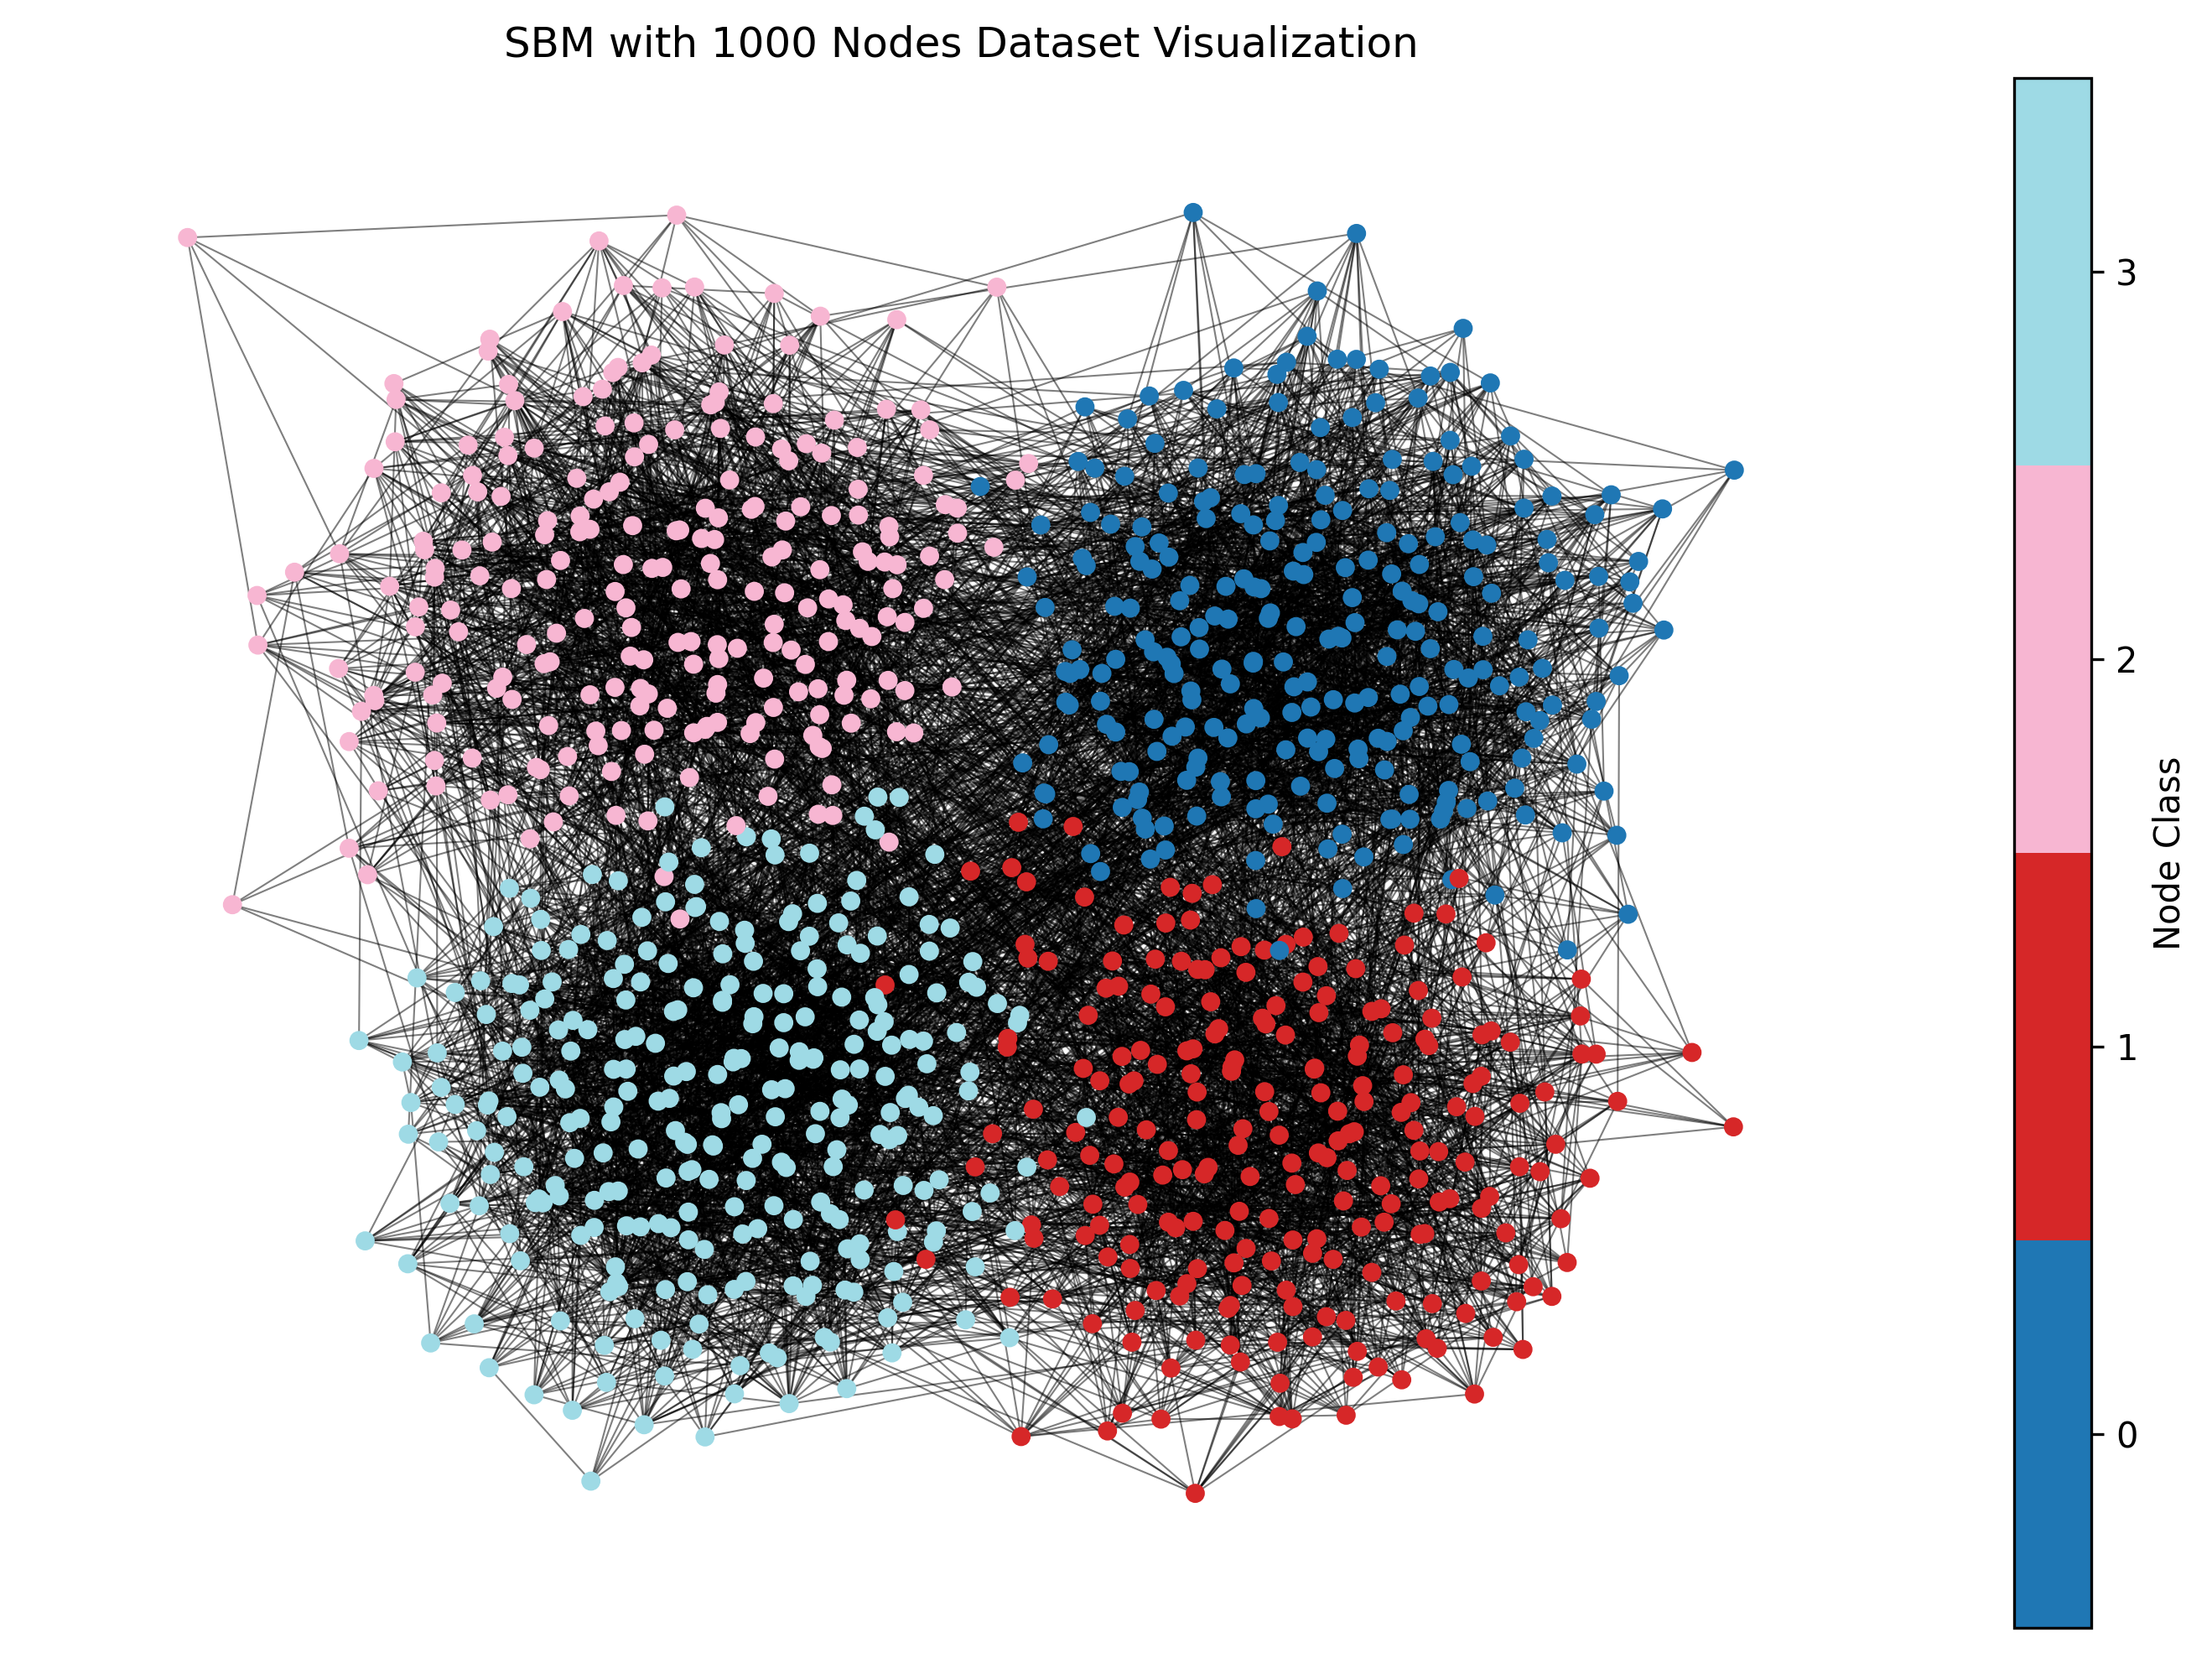
\includegraphics[width=\textwidth]{SBM_with_1000_Nodes_graph.png}
        \caption{SBM dataset with 1000 nodes.}
        \label{fig:sbm_1000}
    \end{subfigure}
    \hfill
    \begin{subfigure}[b]{0.48\textwidth}
        \centering
        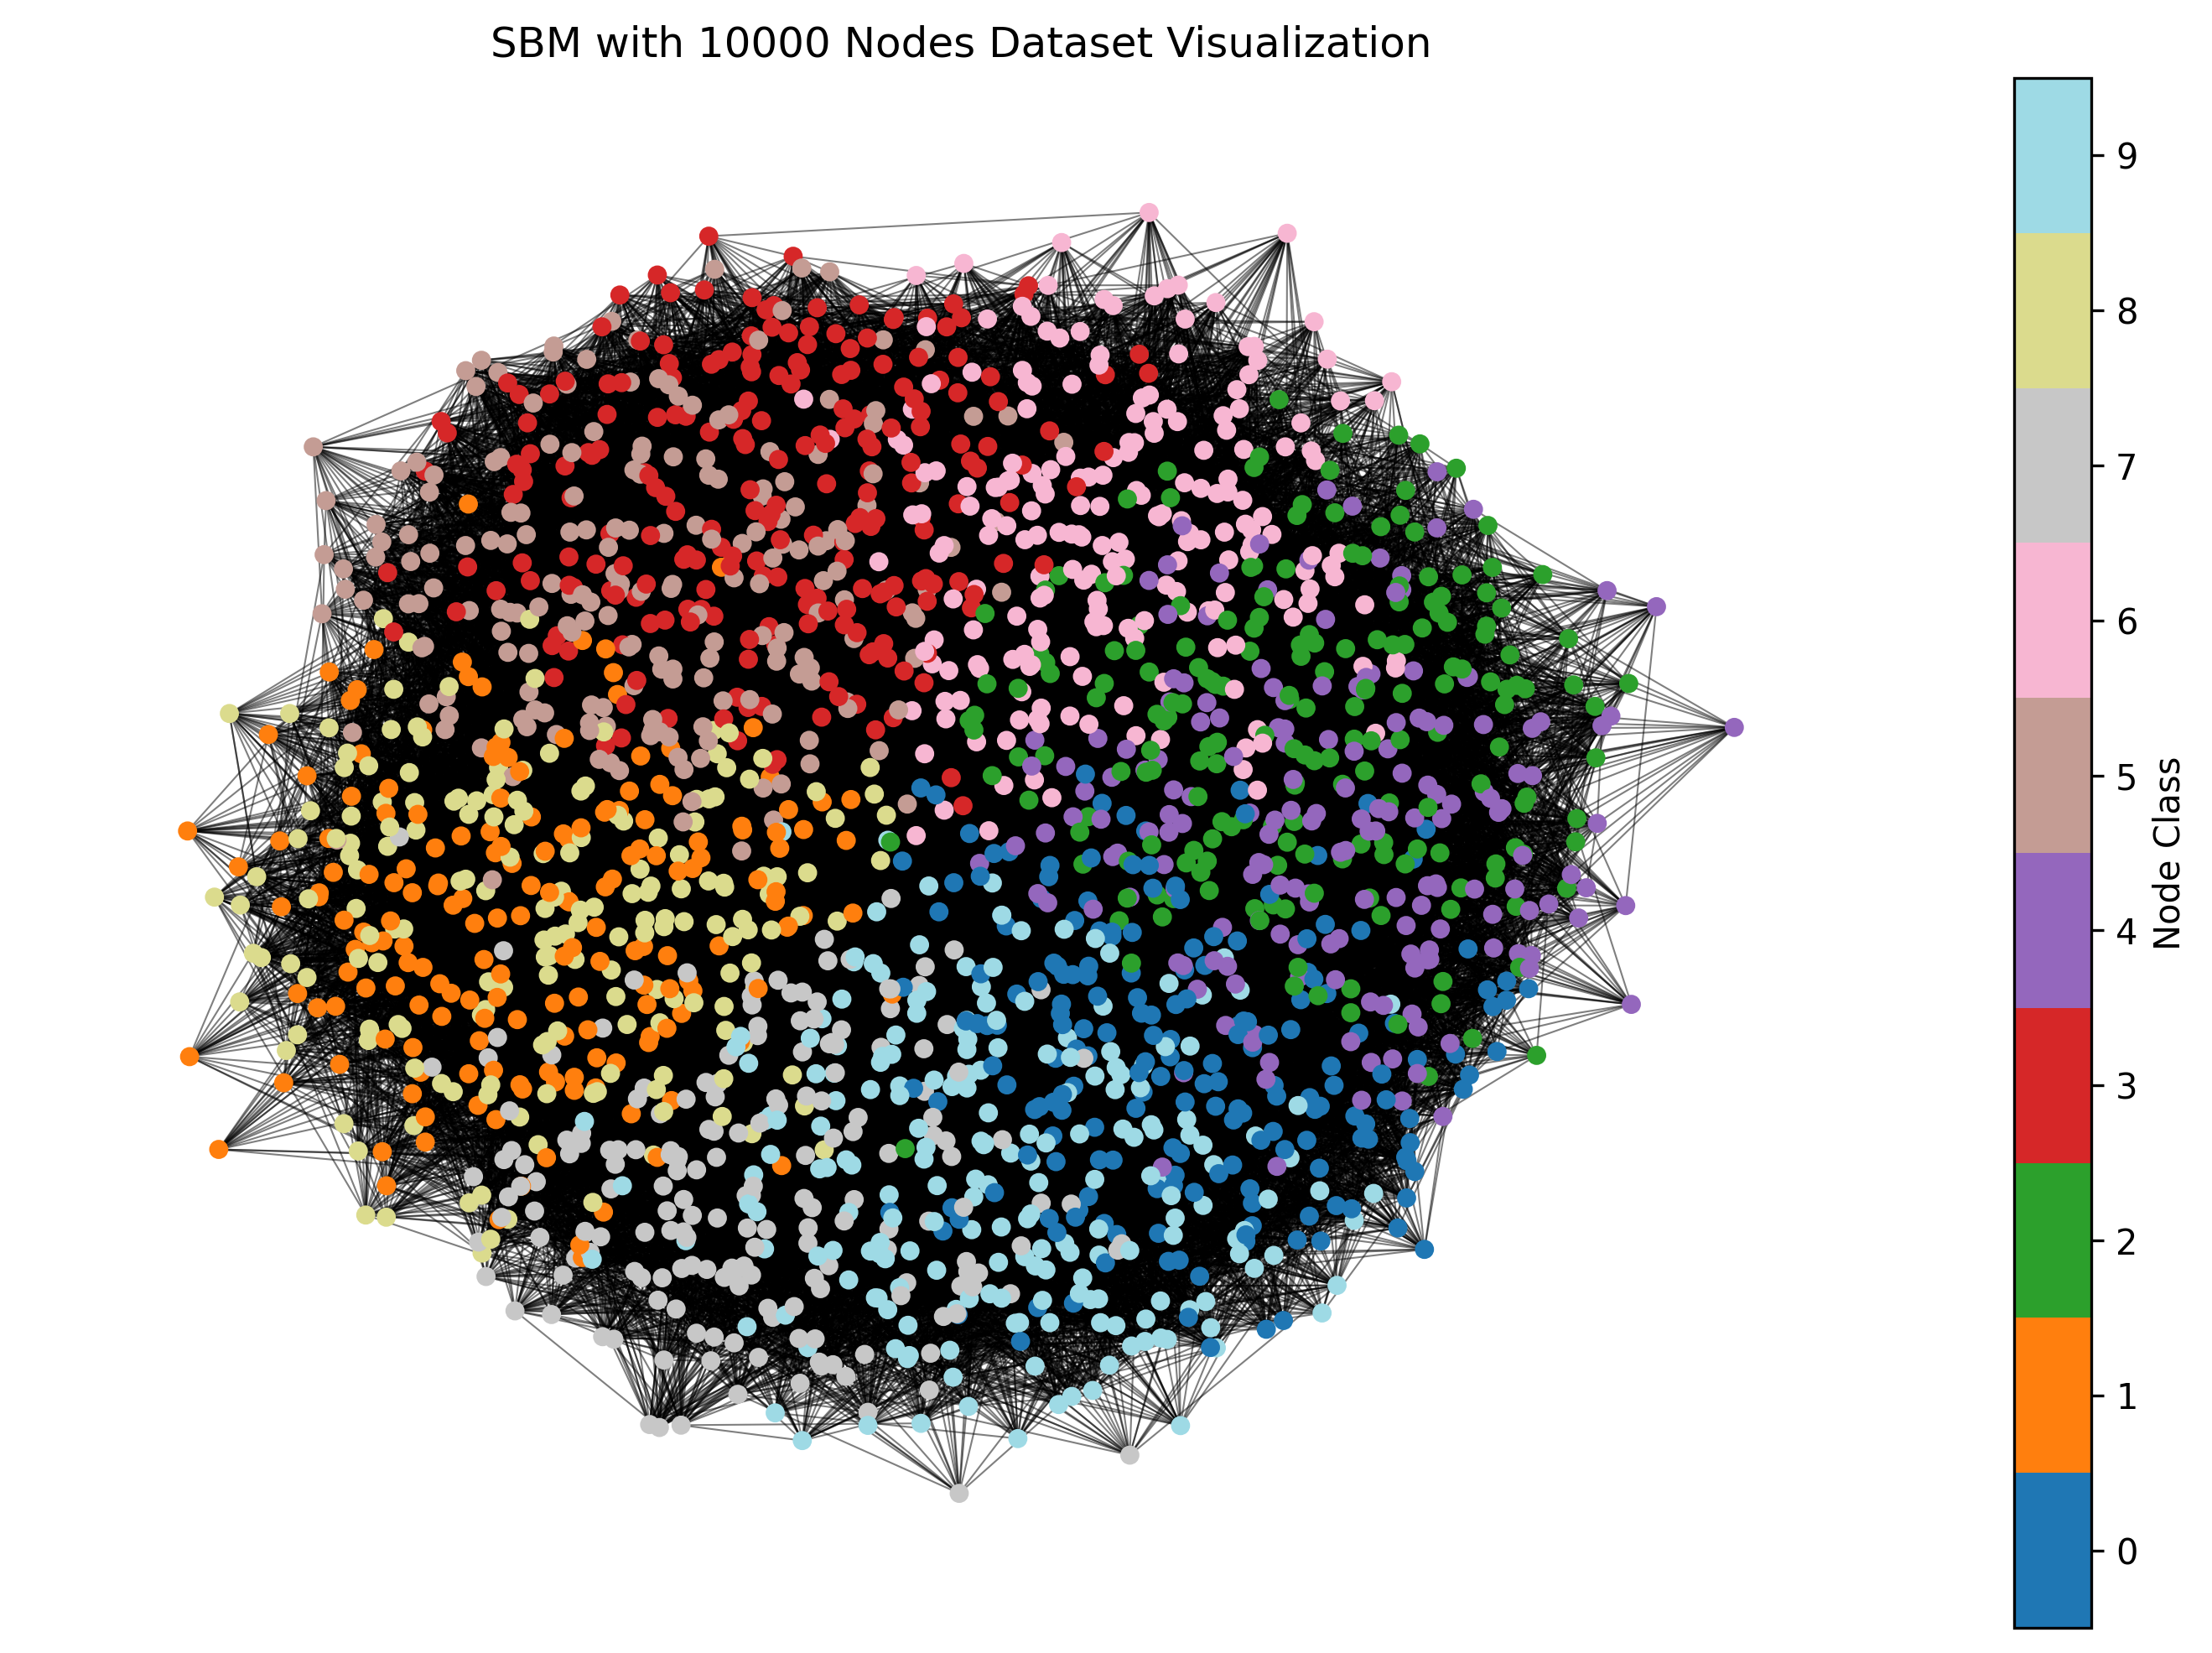
\includegraphics[width=\textwidth]{SBM_with_10000_Nodes_graph.png}
        \caption{SBM dataset with 10,000 nodes.}
        \label{fig:sbm_10000}
    \end{subfigure}
    \caption{Visualization of SBM datasets with 1000 and 10,000 nodes. Node classes are color-coded to highlight community structures.}
    \label{fig:sbm_side_by_side}
\end{figure}

\subsubsection{CORA Dataset}
On the CORA dataset, Neighbor Sampling achieved comparable accuracy to Full-Batch Training but with reduced memory and time requirements. Graph Partitioning demonstrated similar efficiency gains while maintaining high accuracy.

\subsubsection{Reddit Dataset}
On the large-scale Reddit dataset, Full-Batch Training was infeasible due to excessive memory requirements. Both Neighbor Sampling and Graph Partitioning enabled training and achieved competitive accuracy. Among the two, Neighbor Sampling had slightly better training times, while Graph Partitioning excelled in memory optimization.
\begin{figure}[H]
    \centering
    \begin{subfigure}[b]{0.48\textwidth}
        \centering
        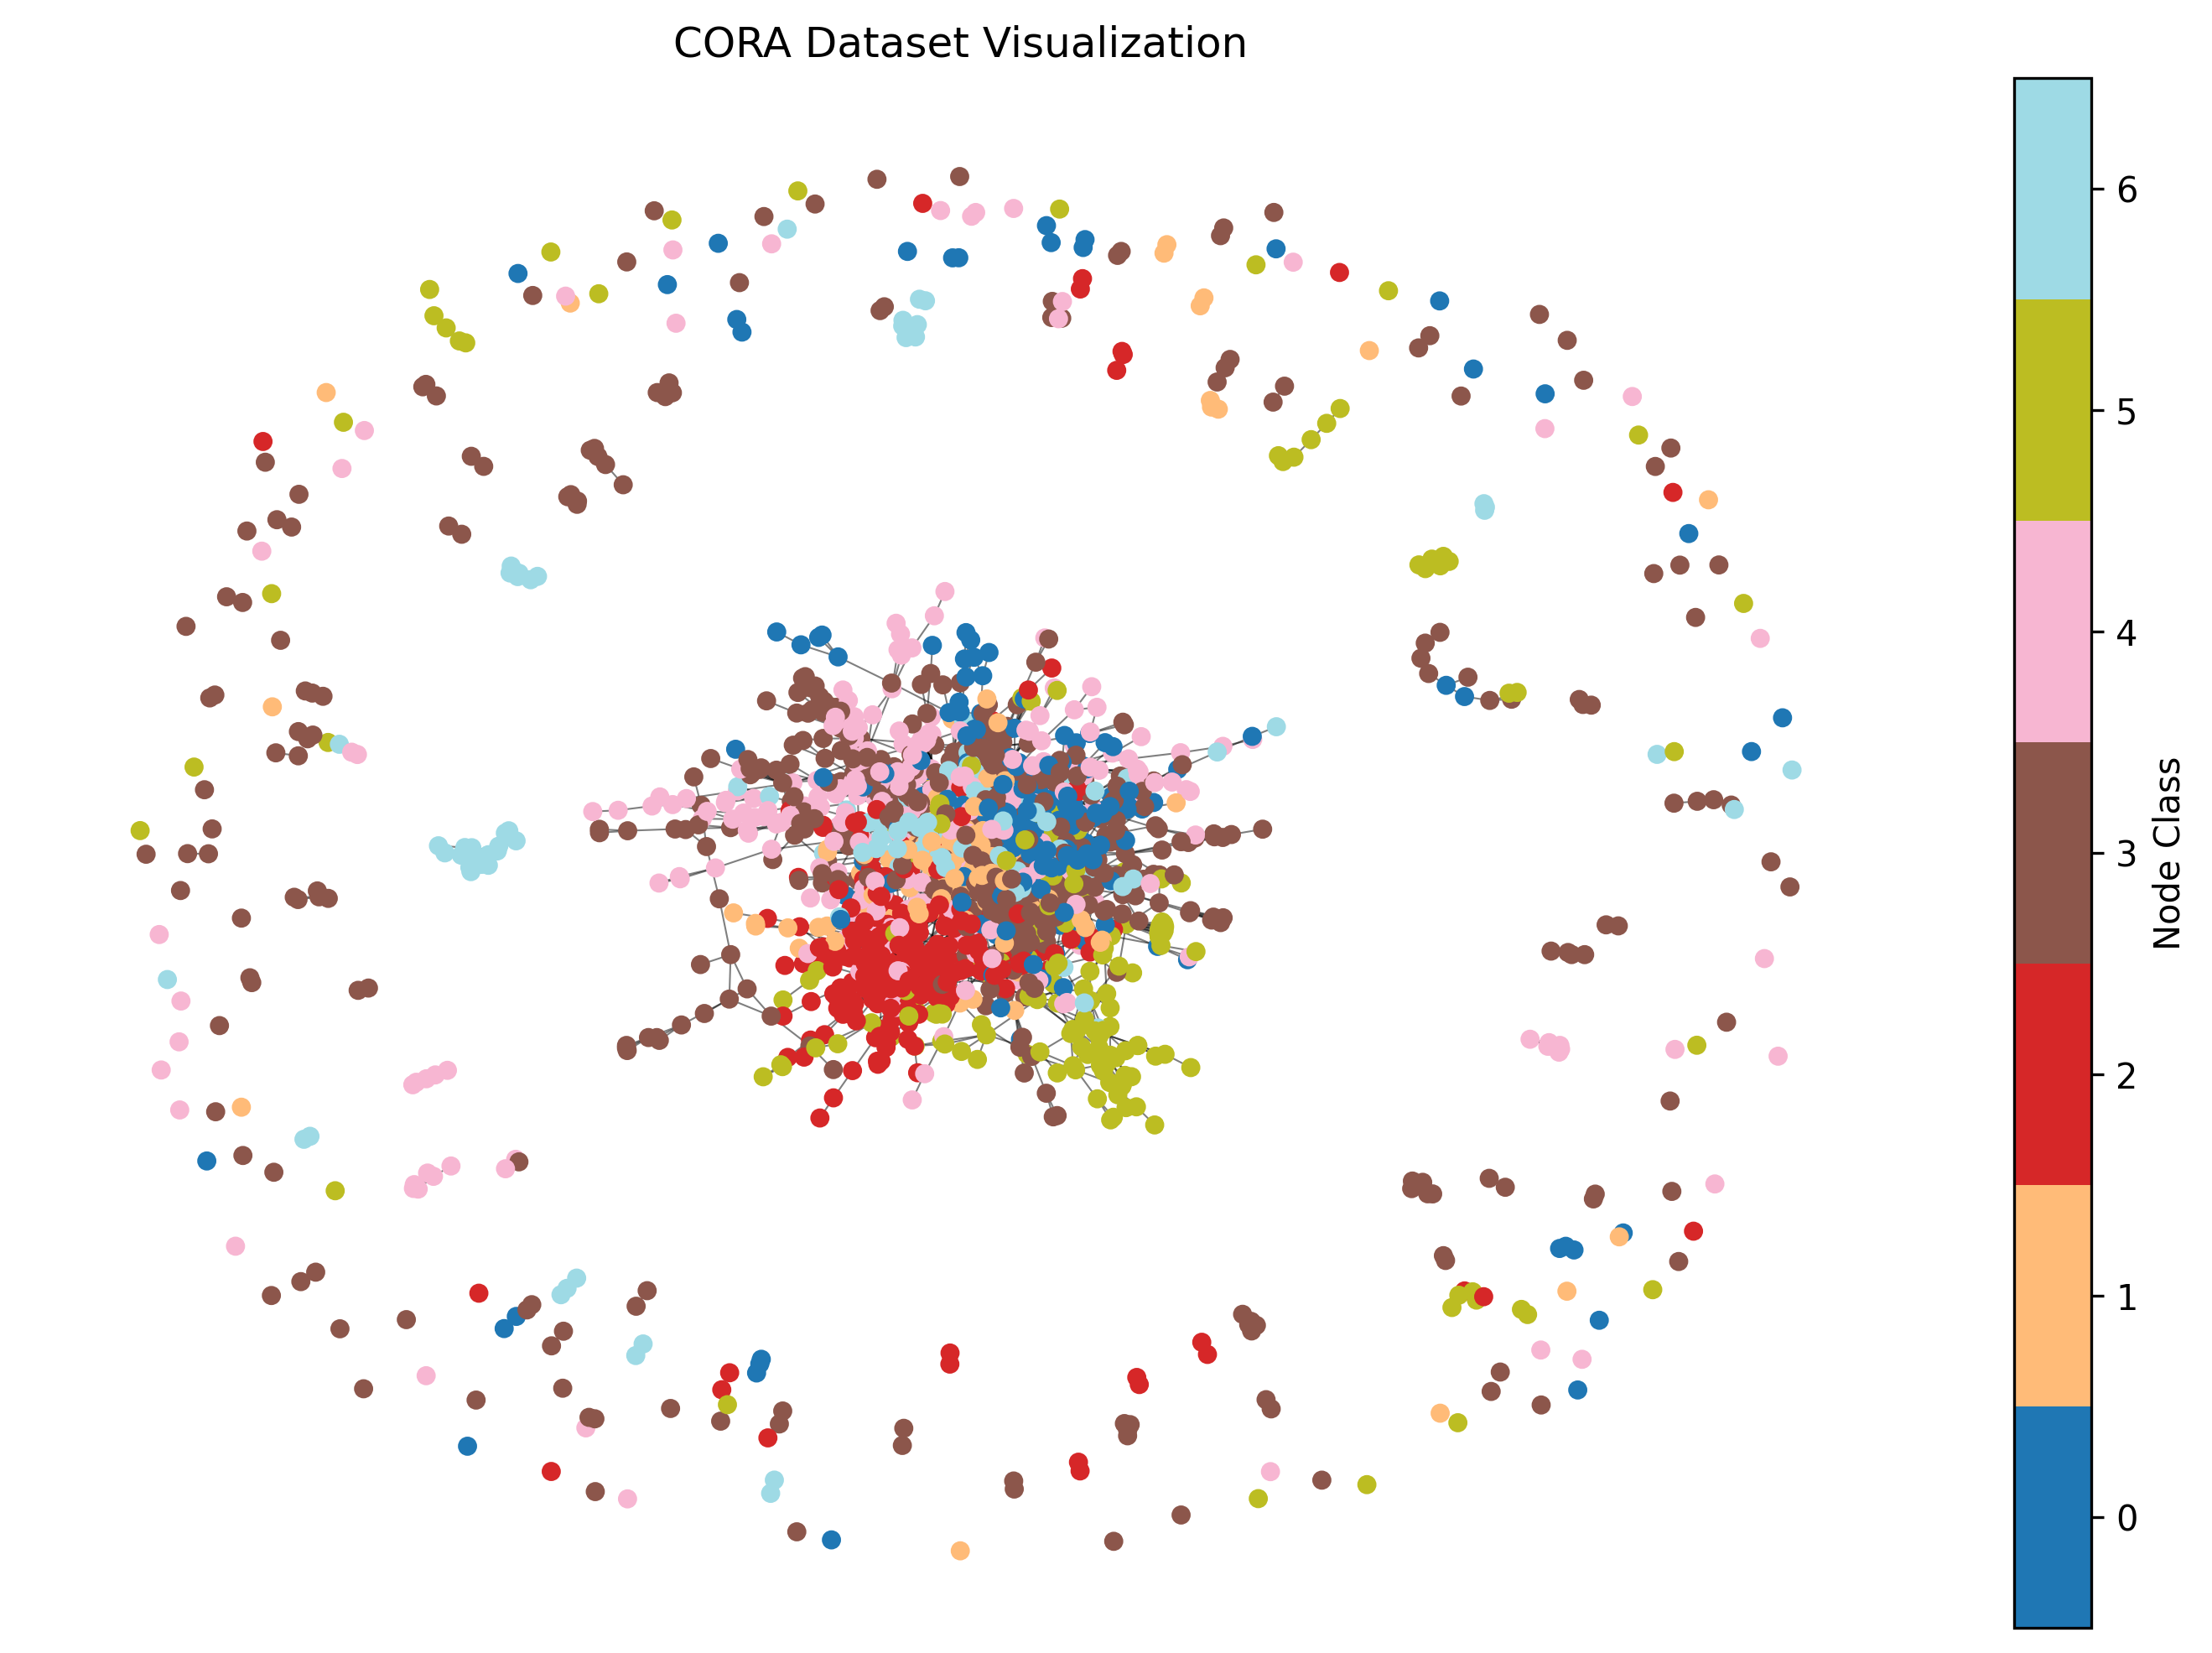
\includegraphics[width=\textwidth]{CORA_graph.png}
        \caption{Visualization of the CORA dataset.}
        \label{fig:cora}
    \end{subfigure}
    \hfill
    \begin{subfigure}[b]{0.48\textwidth}
        \centering
        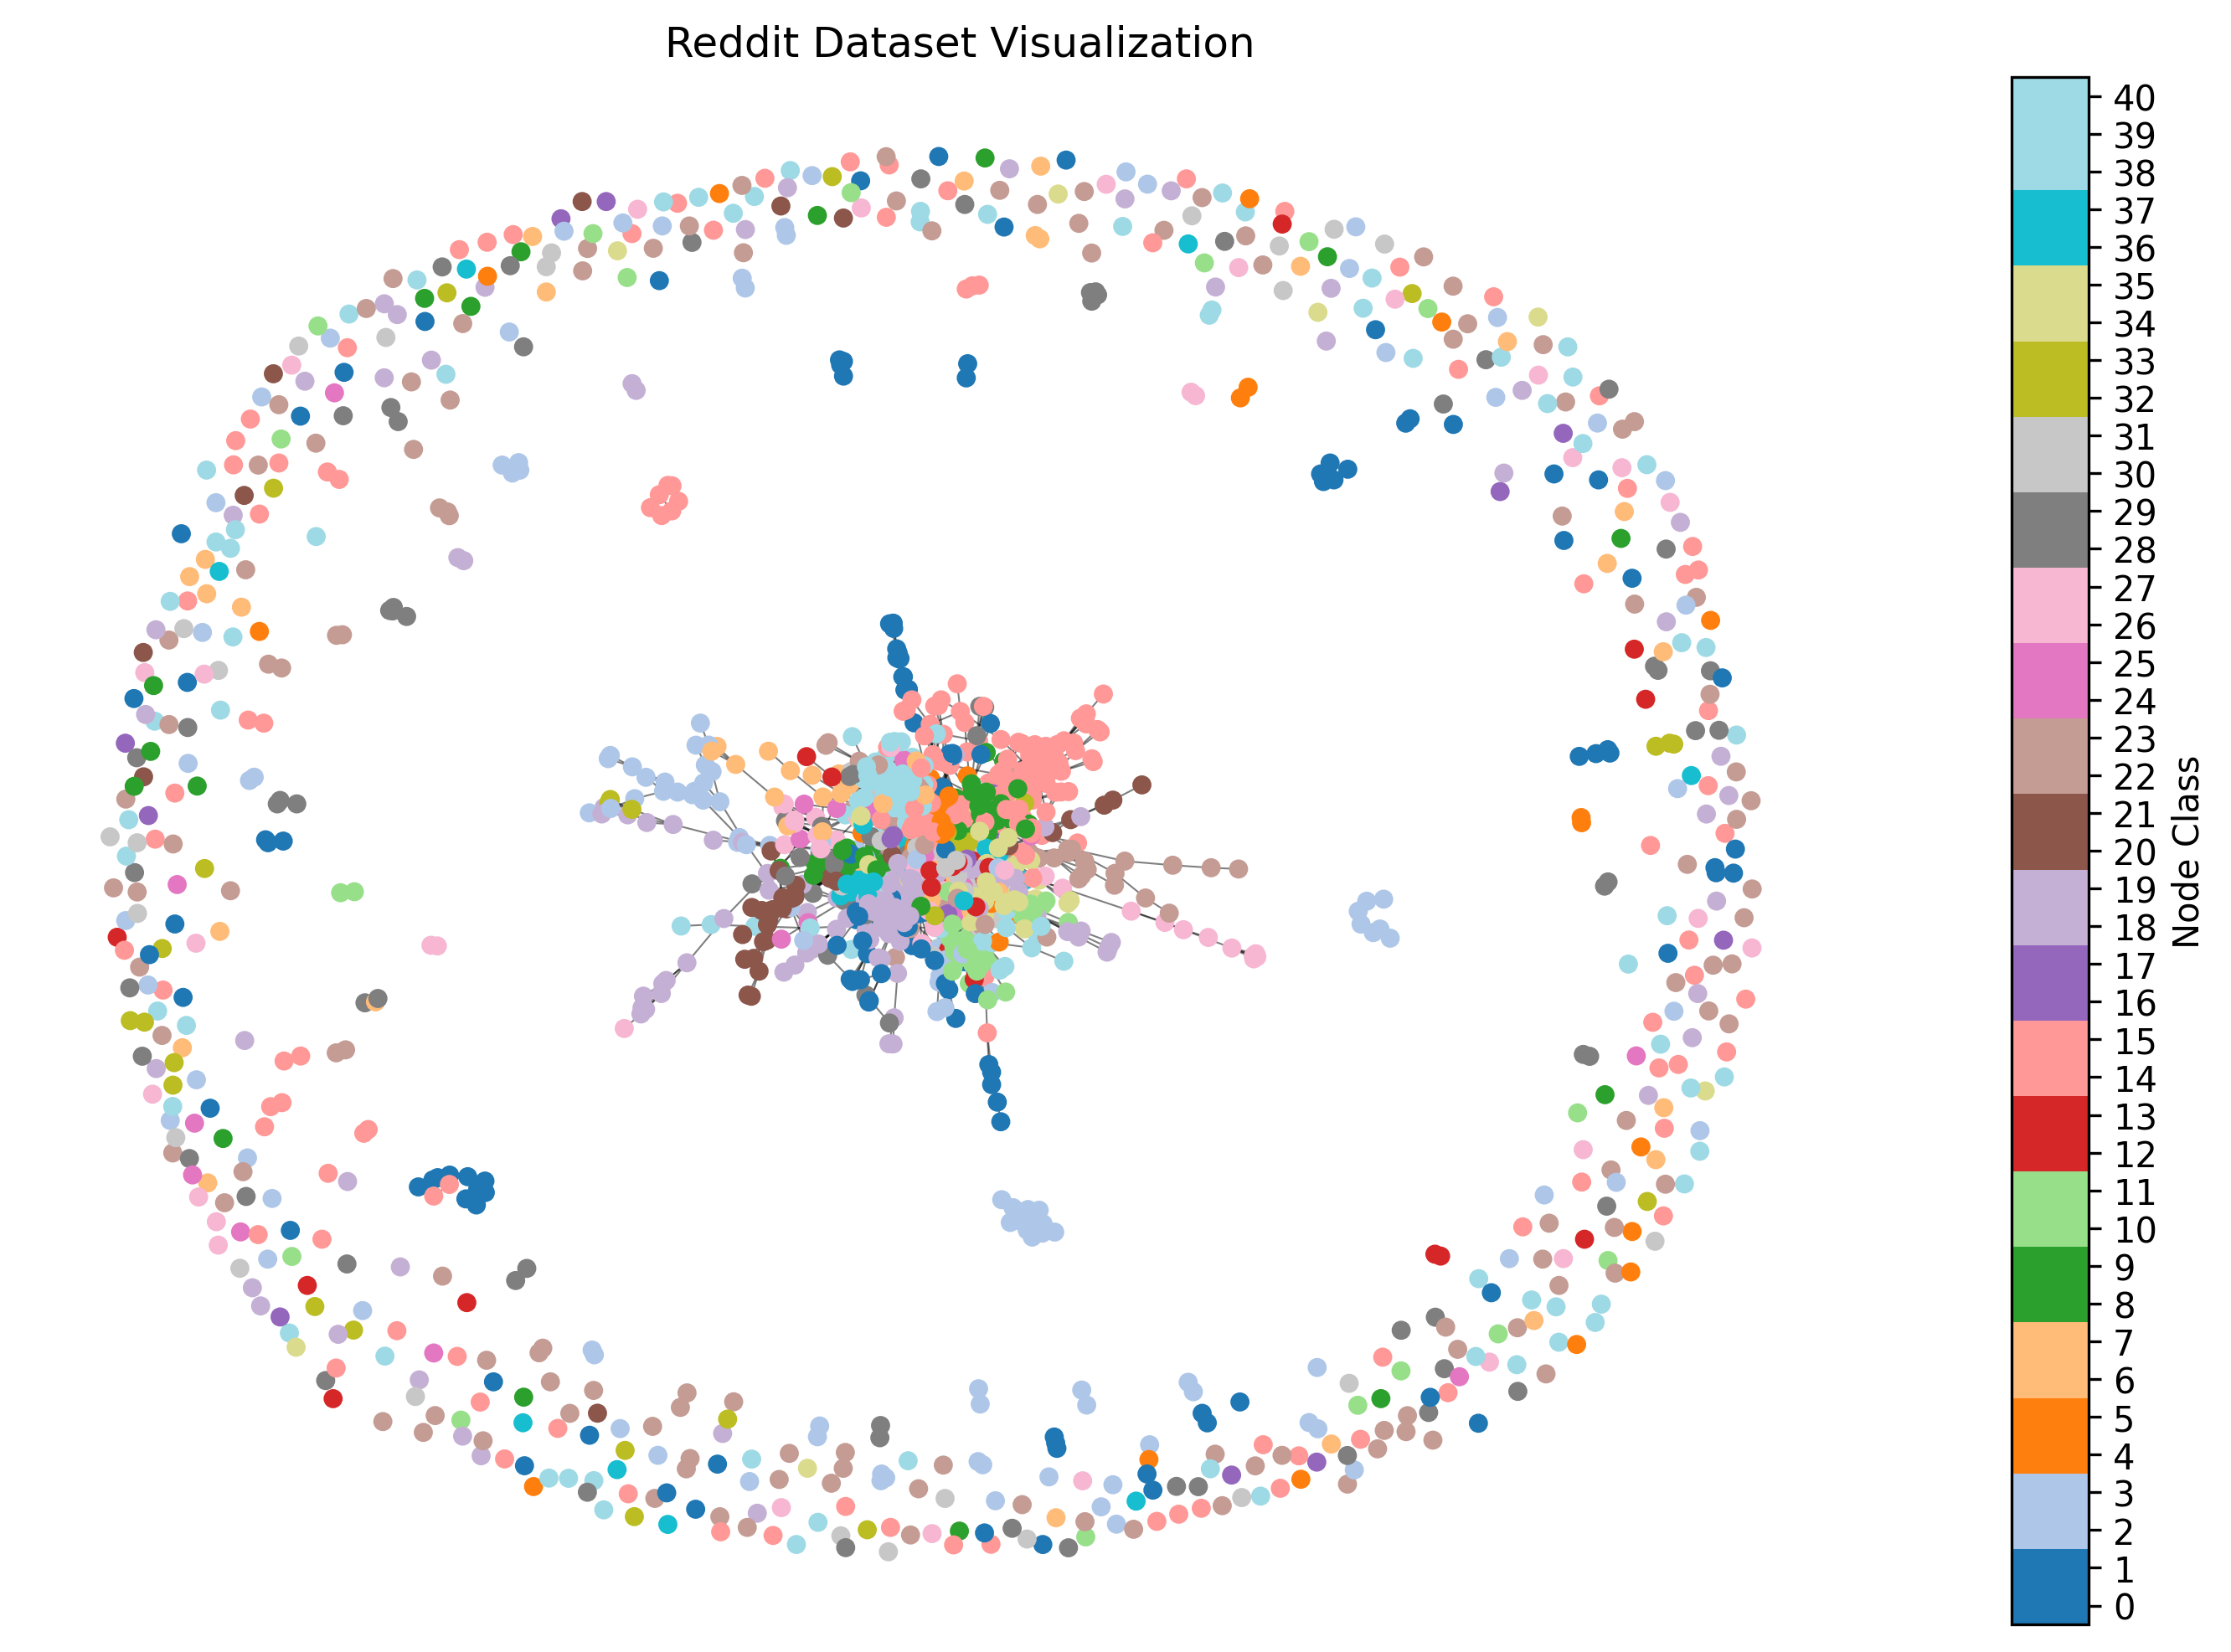
\includegraphics[width=\textwidth]{Reddit_graph.png}
        \caption{Visualization of the Reddit dataset.}
        \label{fig:reddit}
    \end{subfigure}
    \caption{Visualizations of the CORA and Reddit datasets. Node classes are color-coded to represent different communities or research topics.}
    \label{fig:cora_reddit_side_by_side}
\end{figure}

% \subsubsection{Performance on CORA Dataset}

% This subsection compares the performance of different models and training methods on the CORA dataset. The accuracy trends for both training and testing are shown for the various configurations.

% \begin{figure}[H]
%     \centering
%     % First row
%     \begin{subfigure}[b]{0.40\textwidth}
%         \centering
%         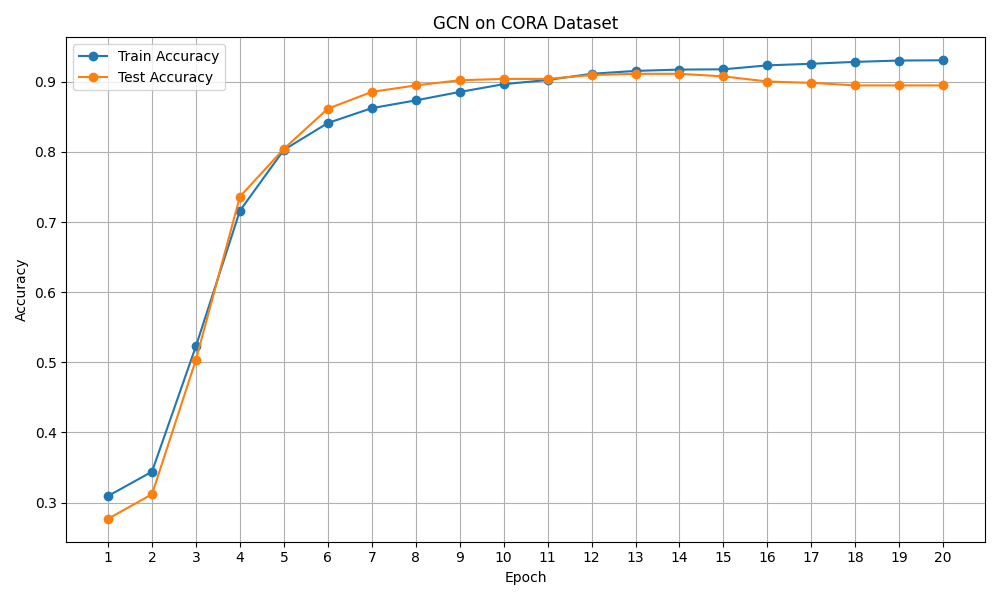
\includegraphics[width=\textwidth]{GCN_on_CORA_Dataset.png}
%         \caption{GCN on CORA Dataset.}
%         \label{fig:gcn_cora}
%     \end{subfigure}
%     \hfill
%     \begin{subfigure}[b]{0.40\textwidth}
%         \centering
%         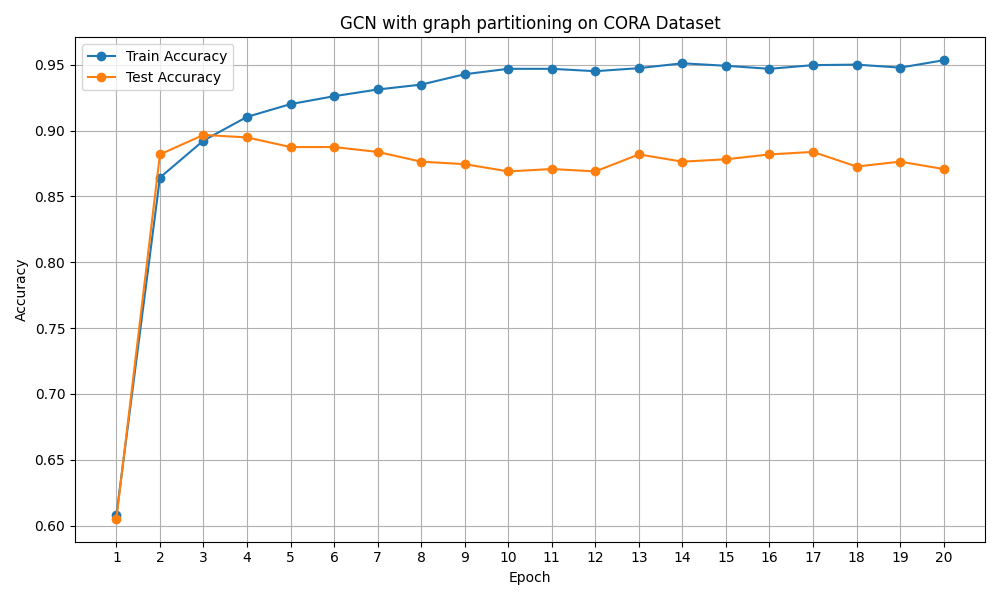
\includegraphics[width=\textwidth]{GCN_with_graph_partitioning_on_CORA_Dataset.png}
%         \caption{GCN with Graph Partitioning on CORA.}
%         \label{fig:gcn_partition_cora}
%     \end{subfigure}

%     % Second row
%     \begin{subfigure}[b]{0.40\textwidth}
%         \centering
%         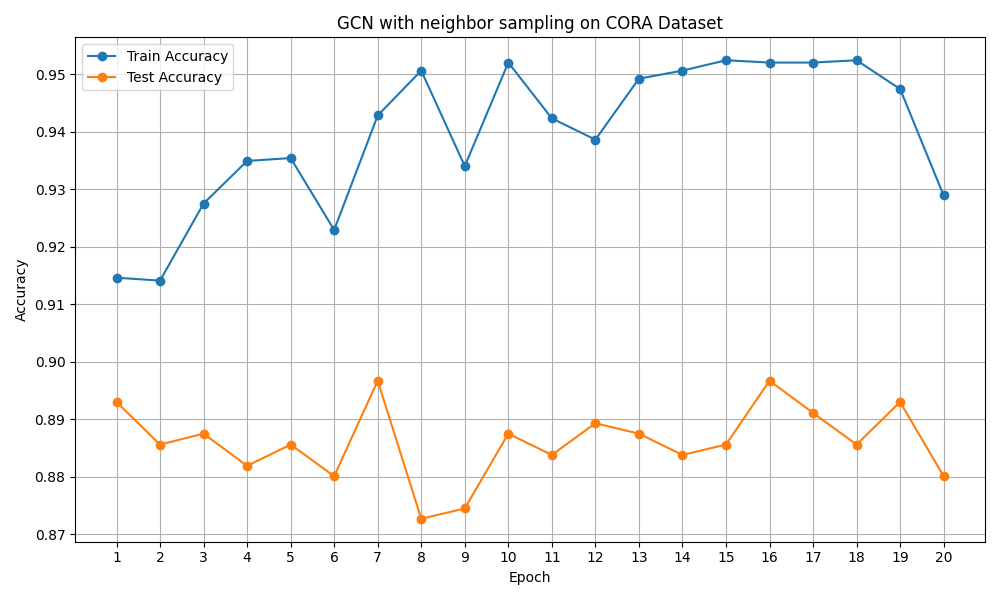
\includegraphics[width=\textwidth]{GCN_with_neighbor_sampling_on_CORA_Dataset.png}
%         \caption{GCN with Neighbor Sampling on CORA.}
%         \label{fig:gcn_neighbor_cora}
%     \end{subfigure}
%     \hfill
%     \begin{subfigure}[b]{0.40\textwidth}
%         \centering
%         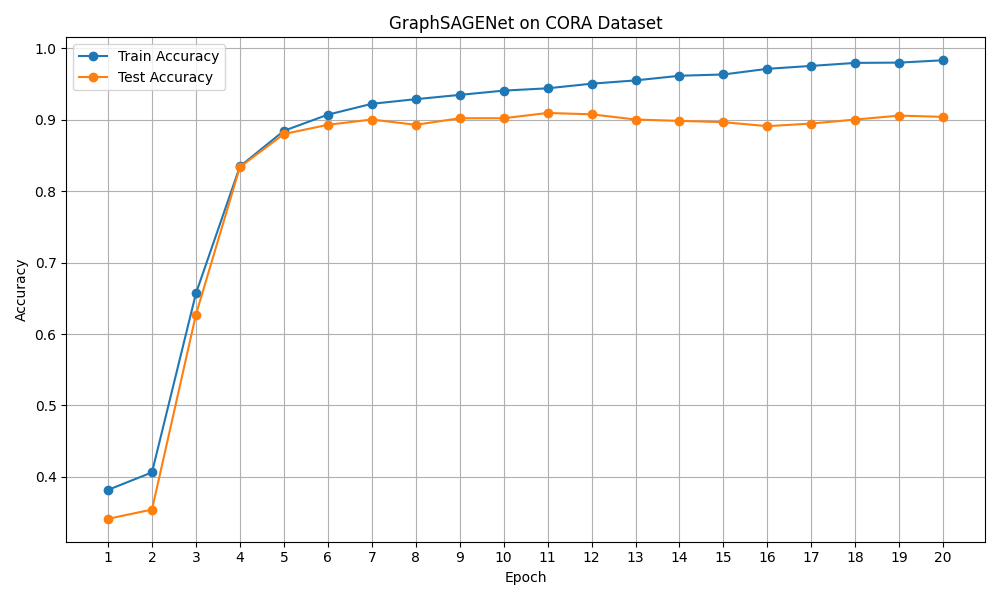
\includegraphics[width=\textwidth]{GraphSAGENet_on_CORA_Dataset.png}
%         \caption{GraphSAGE on CORA Dataset.}
%         \label{fig:graphsage_cora}
%     \end{subfigure}

%     % Third row
%     \begin{subfigure}[b]{0.40\textwidth}
%         \centering
%         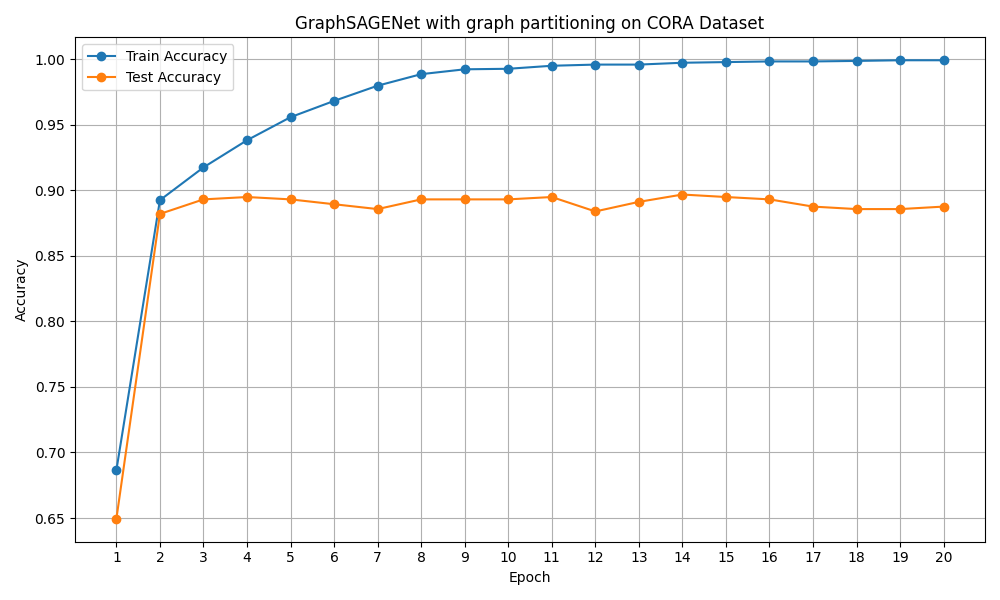
\includegraphics[width=\textwidth]{GraphSAGENet_with_graph_partitioning_on_CORA_Dataset.png}
%         \caption{GraphSAGE with Graph Partitioning on CORA.}
%         \label{fig:graphsage_partition_cora}
%     \end{subfigure}
%     \hfill
%     \begin{subfigure}[b]{0.40\textwidth}
%         \centering
%         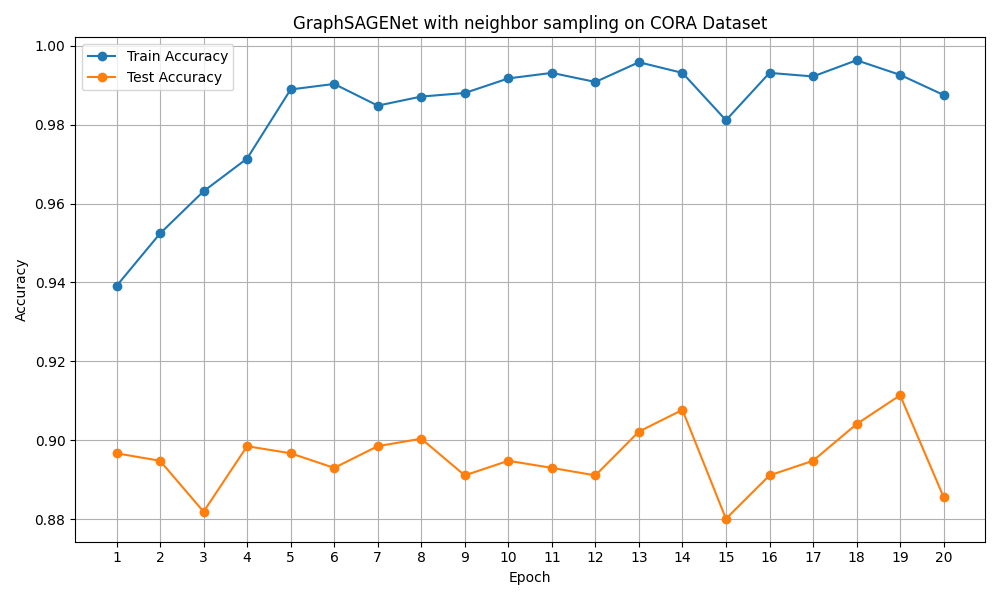
\includegraphics[width=\textwidth]{GraphSAGENet_with_neighbor_sampling_on_CORA_Dataset.png}
%         \caption{GraphSAGE with Neighbor Sampling on CORA.}
%         \label{fig:graphsage_neighbor_cora}
%     \end{subfigure}

%     \caption{Performance comparison on the CORA dataset for GCN and GraphSAGE models under different training strategies: Full-Batch, Graph Partitioning, and Neighbor Sampling.}
%     \label{fig:performance_cora}
% \end{figure}

% \subsubsection{Performance on Reddit Dataset}

% This subsection compares the performance of different models and training methods on the Reddit dataset. The accuracy trends for both training and testing are shown for the various configurations.

% \begin{figure}[H]
%     \centering
%     % First row
%     \begin{subfigure}[b]{0.68\textwidth}
%         \centering
%         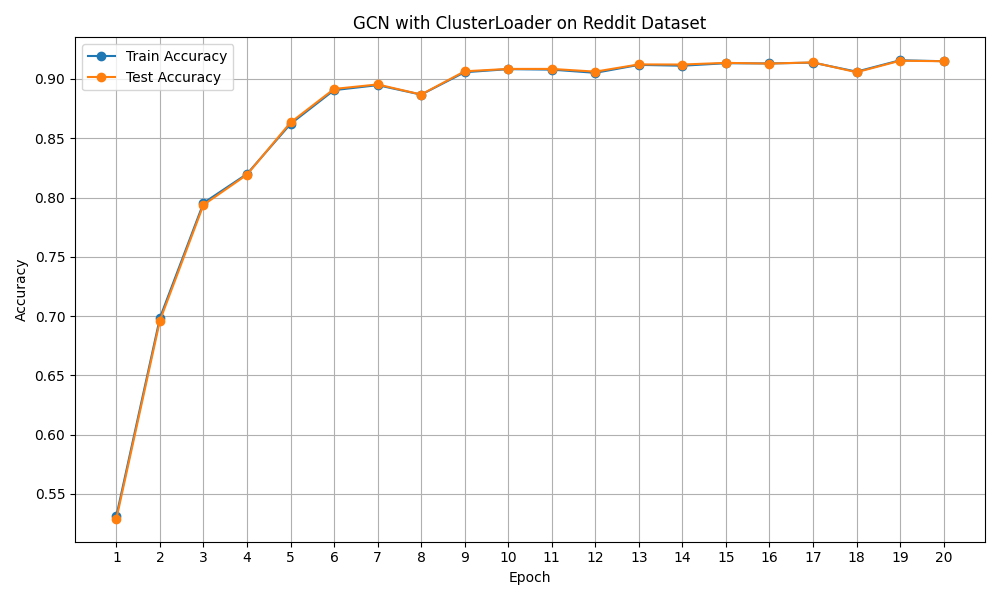
\includegraphics[width=\textwidth]{GCN_with_ClusterLoader_on_Reddit_Dataset.png}
%         \caption{GCN with ClusterLoader on Reddit Dataset.}
%         \label{fig:gcn_clusterloader_reddit}
%     \end{subfigure}
%     \hfill
%     \begin{subfigure}[b]{0.68\textwidth}
%         \centering
%         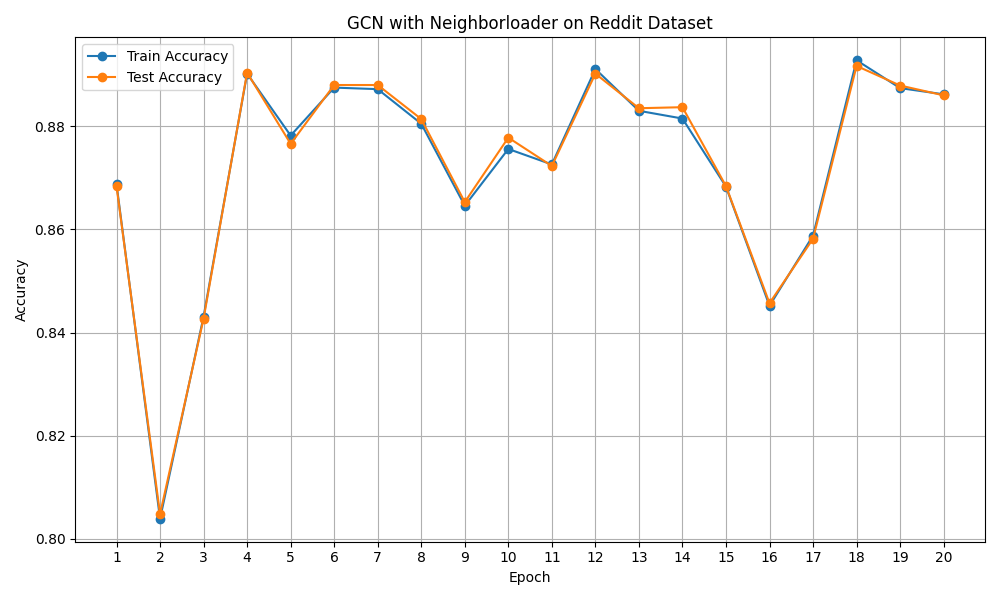
\includegraphics[width=\textwidth]{GCN_with_Neighborloader_on_Reddit_Dataset.png}
%         \caption{GCN with Neighborloader on Reddit Dataset.}
%         \label{fig:gcn_neighborloader_reddit}
%     \end{subfigure}
%      \hfill
%     % Second row
%     \begin{subfigure}[b]{0.68\textwidth}
%         \centering
%         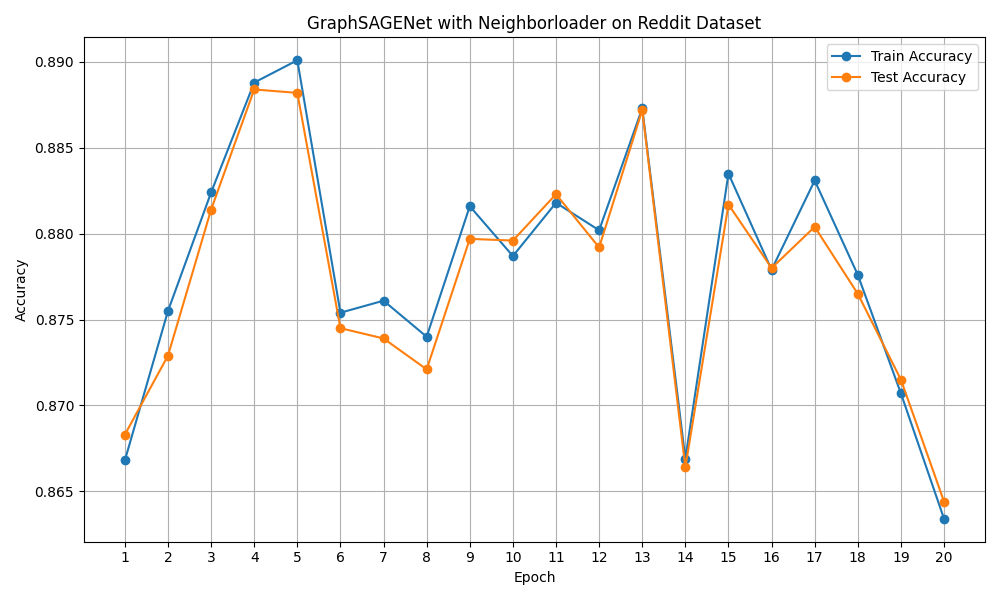
\includegraphics[width=\textwidth]{GraphSAGENet_with_Neighborloader_on_Reddit_Dataset.png}
%         \caption{GraphSAGE with Neighborloader on Reddit Dataset.}
%         \label{fig:graphsage_neighborloader_reddit}
%     \end{subfigure}
%     \caption{Performance comparison on the Reddit dataset for GCN and GraphSAGE models under different training strategies: ClusterLoader and Neighborloader.}
%     \label{fig:performance_reddit}
% \end{figure}

% \subsubsection{Performance on SBM Dataset (1000 Nodes)}

% This subsection compares the performance of different models and training methods on the SBM dataset with 1000 nodes. The accuracy trends for both training and testing are shown for the various configurations. [Figure~\ref{fig:graphsage_neighbor_sbm_1000}]

% \begin{figure}[H]
%     \centering
%     % First row
%     \begin{subfigure}[b]{0.48\textwidth}
%         \centering
%         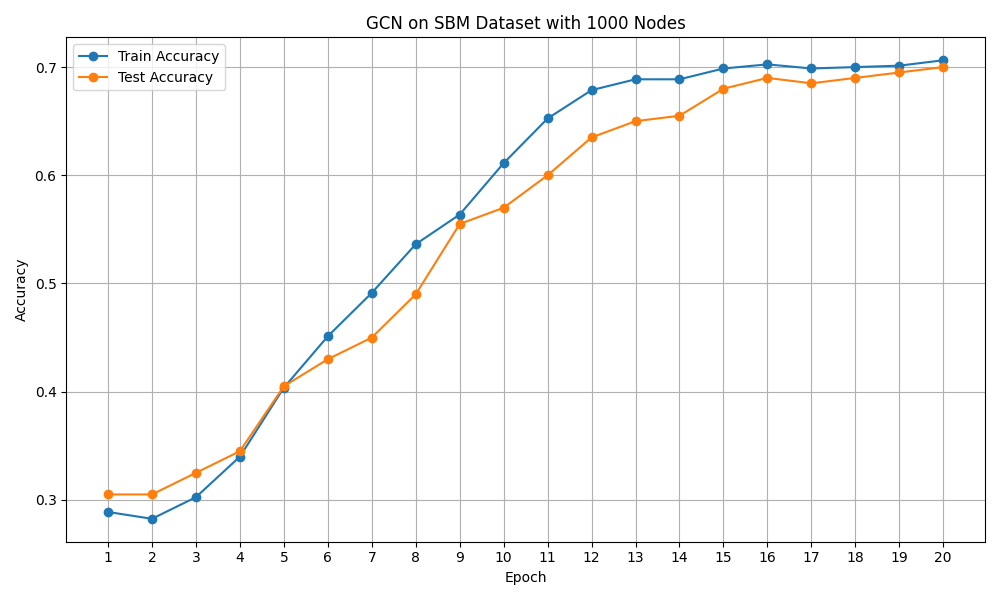
\includegraphics[width=\textwidth]{GCN_on_SBM_Dataset_with_1000_Nodes.png}
%         \caption{GCN on SBM Dataset.}
%         \label{fig:gcn_sbm_1000}
%     \end{subfigure}
%     \hfill
%     \begin{subfigure}[b]{0.48\textwidth}
%         \centering
%         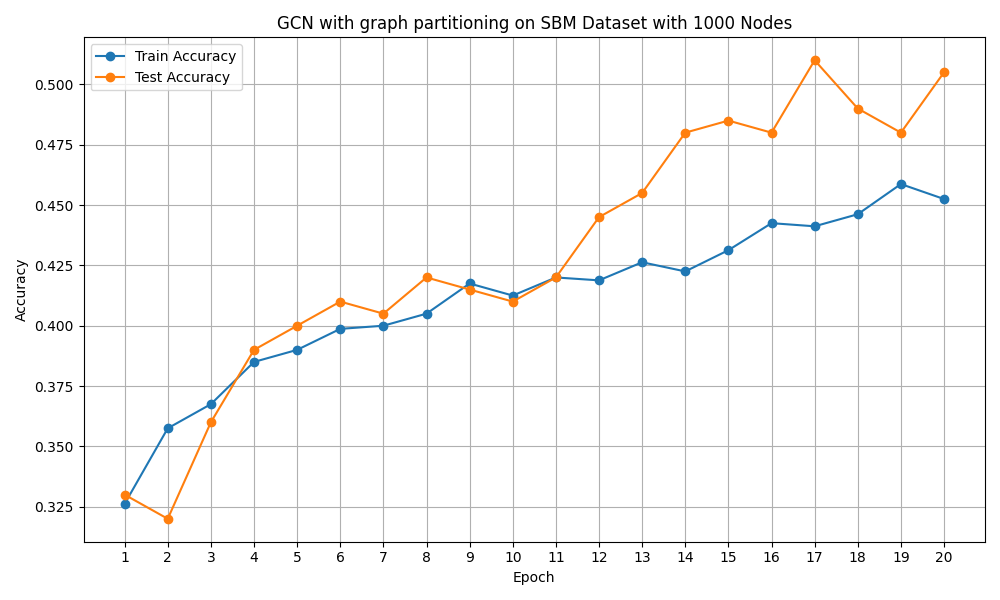
\includegraphics[width=\textwidth]{GCN_with_graph_partitioning_on_SBM_Dataset_with_1000_Nodes.png}
%         \caption{GCN with Graph Partitioning on SBM Dataset.}
%         \label{fig:gcn_partition_sbm_1000}
%     \end{subfigure}

%     % Second row
%     \begin{subfigure}[b]{0.48\textwidth}
%         \centering
%         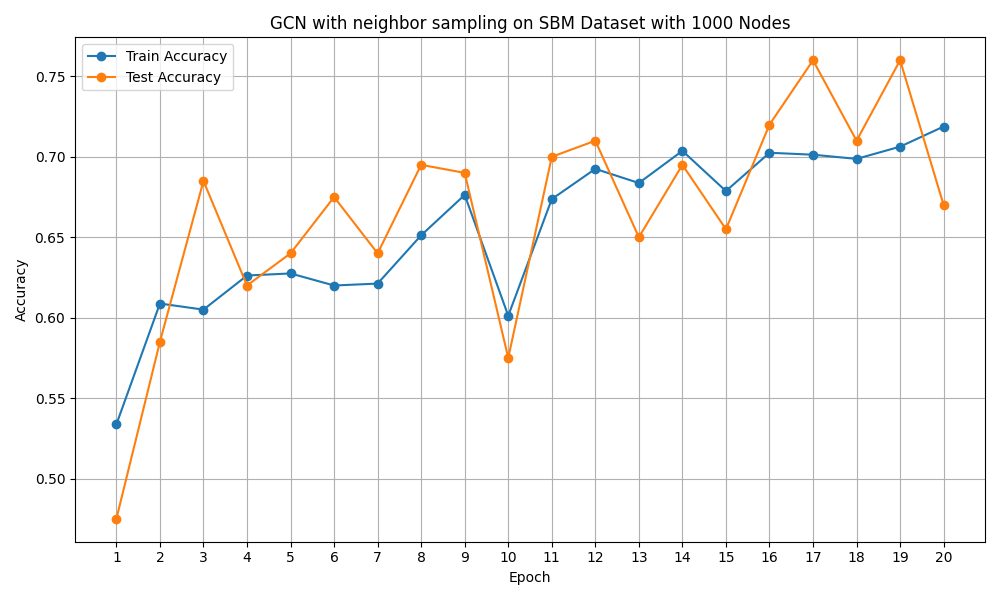
\includegraphics[width=\textwidth]{GCN_with_neighbor_sampling_on_SBM_Dataset_with_1000_Nodes.png}
%         \caption{GCN with Neighbor Sampling on SBM Dataset.}
%         \label{fig:gcn_neighbor_sbm_1000}
%     \end{subfigure}
%     \hfill
%     \begin{subfigure}[b]{0.48\textwidth}
%         \centering
%         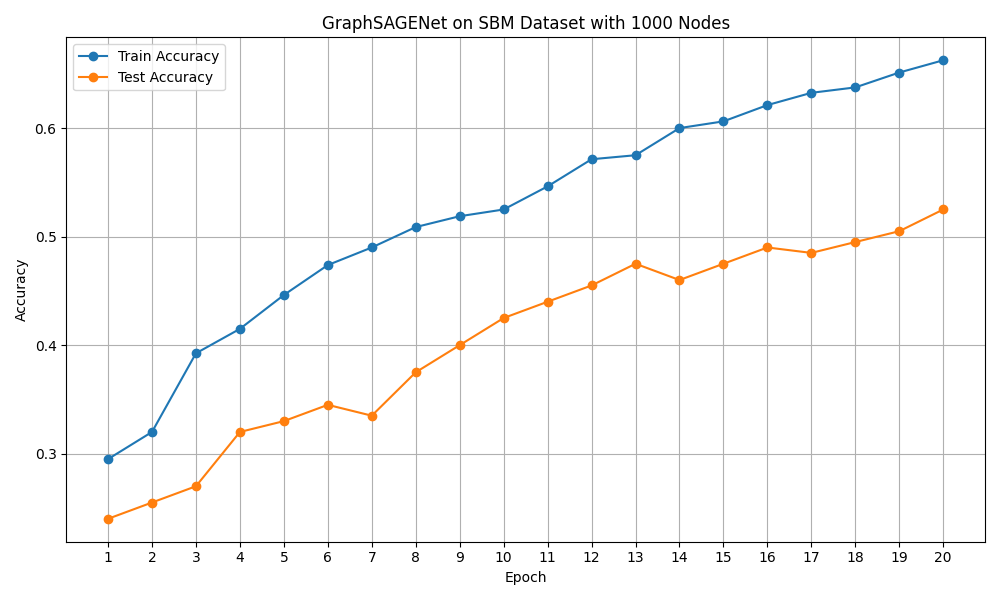
\includegraphics[width=\textwidth]{GraphSAGENet_on_SBM_Dataset_with_1000_Nodes.png}
%         \caption{GraphSAGE on SBM Dataset.}
%         \label{fig:graphsage_sbm_1000}
%     \end{subfigure}

%     % Third row
%     \begin{subfigure}[b]{0.48\textwidth}
%         \centering
%         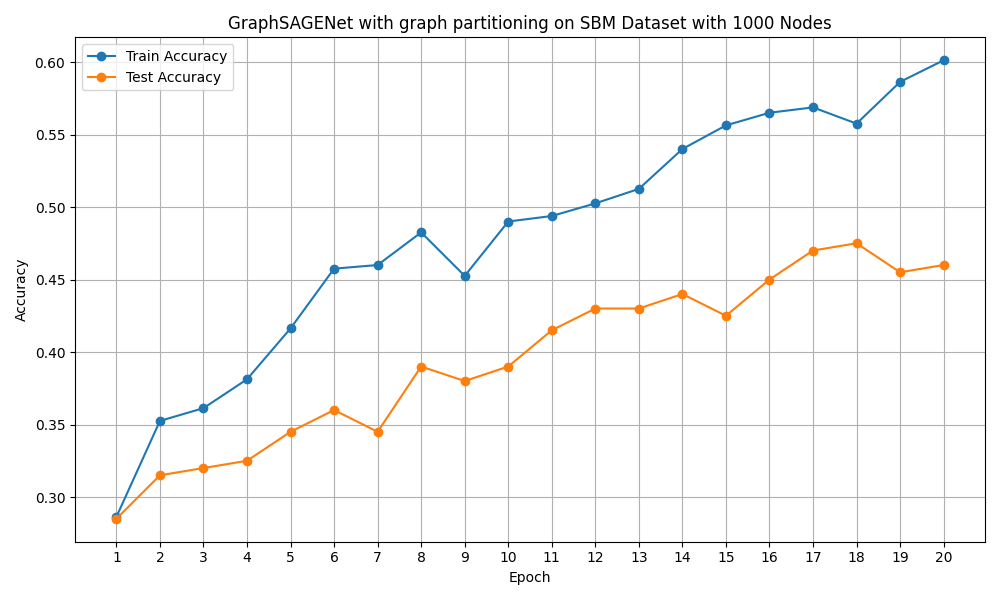
\includegraphics[width=\textwidth]{GraphSAGENet_with_graph_partitioning_on_SBM_Dataset_with_1000_Nodes.png}
%         \caption{GraphSAGE with Graph Partitioning on SBM Dataset.}
%         \label{fig:graphsage_partition_sbm_1000}
%     \end{subfigure}
%     \hfill
%     \begin{subfigure}[b]{0.48\textwidth}
%         \centering
%         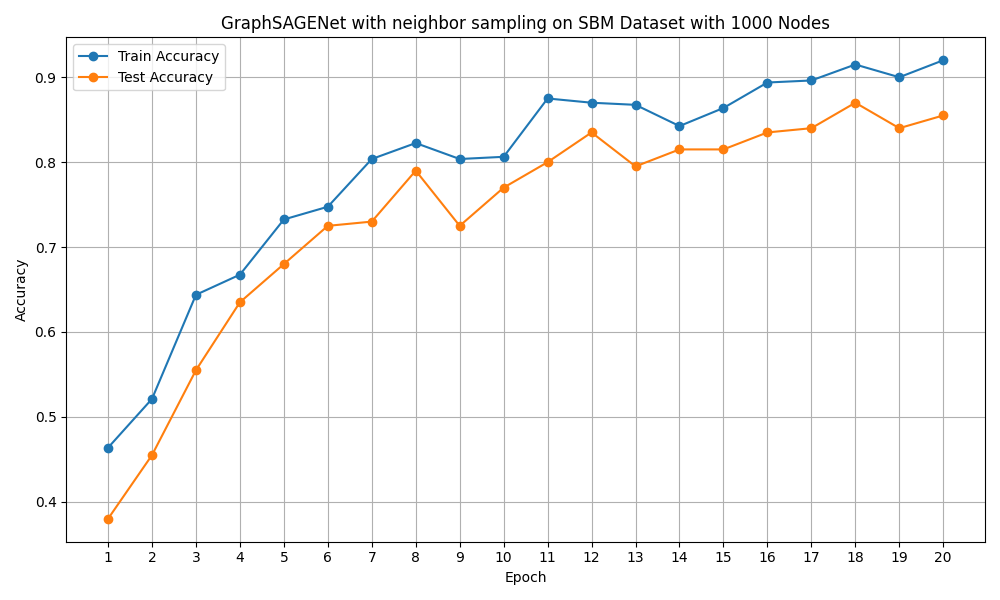
\includegraphics[width=\textwidth]{GraphSAGENet_with_neighbor_sampling_on_SBM_Dataset_with_1000_Nodes.png}
%         \caption{GraphSAGE with Neighbor Sampling on SBM Dataset.}
%         \label{fig:graphsage_neighbor_sbm_1000}
%     \end{subfigure}

%     \caption{Performance comparison on the SBM dataset with 1000 nodes for GCN and GraphSAGE models under different training strategies: Full-Batch, Graph Partitioning, and Neighbor Sampling.}
%     \label{fig:performance_sbm_1000}
% \end{figure}

% \subsubsection{Performance on SBM Dataset (10,000 Nodes)}

% This subsection compares the performance of different models and training methods on the SBM dataset with 10,000 nodes. The accuracy trends for both training and testing are shown for the various configurations. [Figure~\ref{fig:graphsage_neighbor_sbm_10000}]

% \begin{figure}[H]
%     \centering
%     % First row
%     \begin{subfigure}[b]{0.48\textwidth}
%         \centering
%         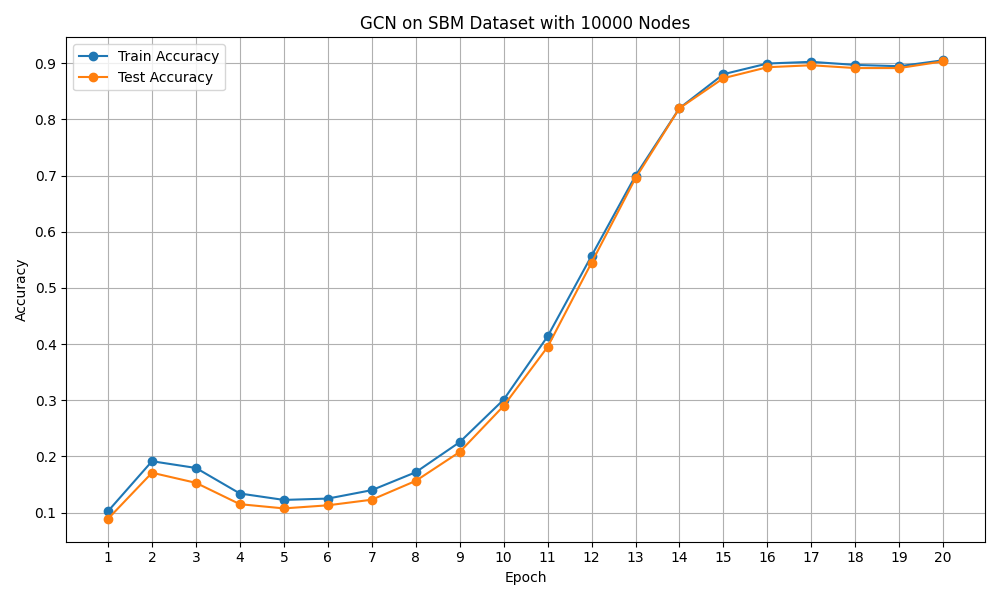
\includegraphics[width=\textwidth]{GCN_on_SBM_Dataset_with_10000_Nodes.png}
%         \caption{GCN on SBM Dataset.}
%         \label{fig:gcn_sbm_10000}
%     \end{subfigure}
%     \hfill
%     \begin{subfigure}[b]{0.48\textwidth}
%         \centering
%         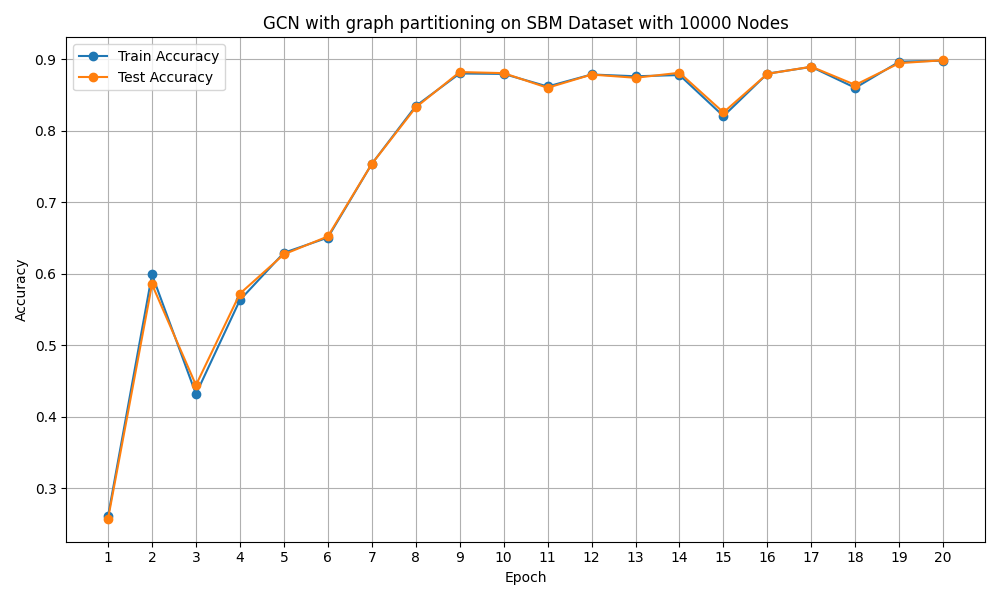
\includegraphics[width=\textwidth]{GCN_with_graph_partitioning_on_SBM_Dataset_with_10000_Nodes.png}
%         \caption{GCN with Graph Partitioning on SBM Dataset.}
%         \label{fig:gcn_partition_sbm_10000}
%     \end{subfigure}

%     % Second row
%     \begin{subfigure}[b]{0.48\textwidth}
%         \centering
%         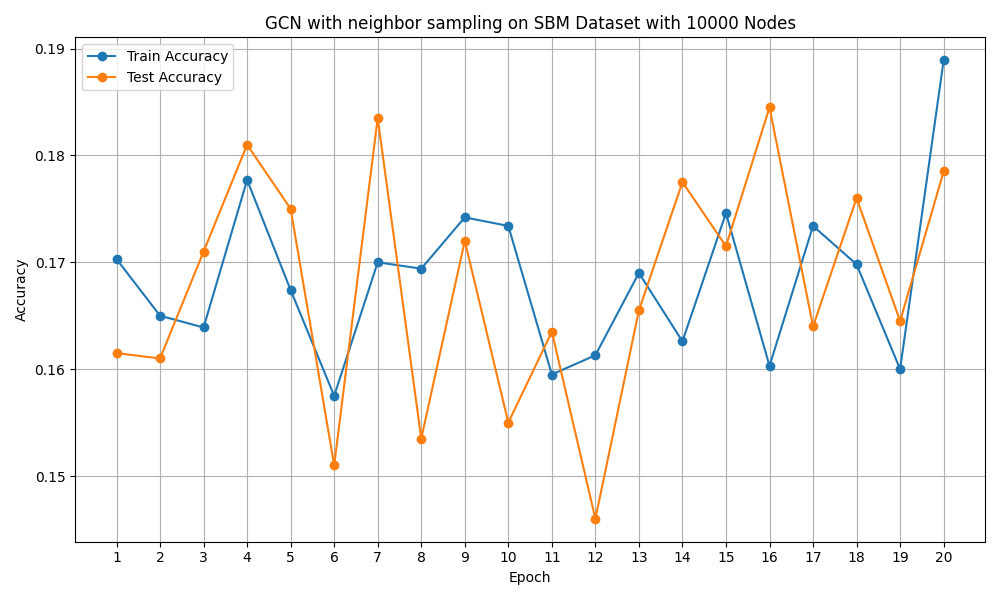
\includegraphics[width=\textwidth]{GCN_with_neighbor_sampling_on_SBM_Dataset_with_10000_Nodes.png}
%         \caption{GCN with Neighbor Sampling on SBM Dataset.}
%         \label{fig:gcn_neighbor_sbm_10000}
%     \end{subfigure}
%     \hfill
%     \begin{subfigure}[b]{0.48\textwidth}
%         \centering
%         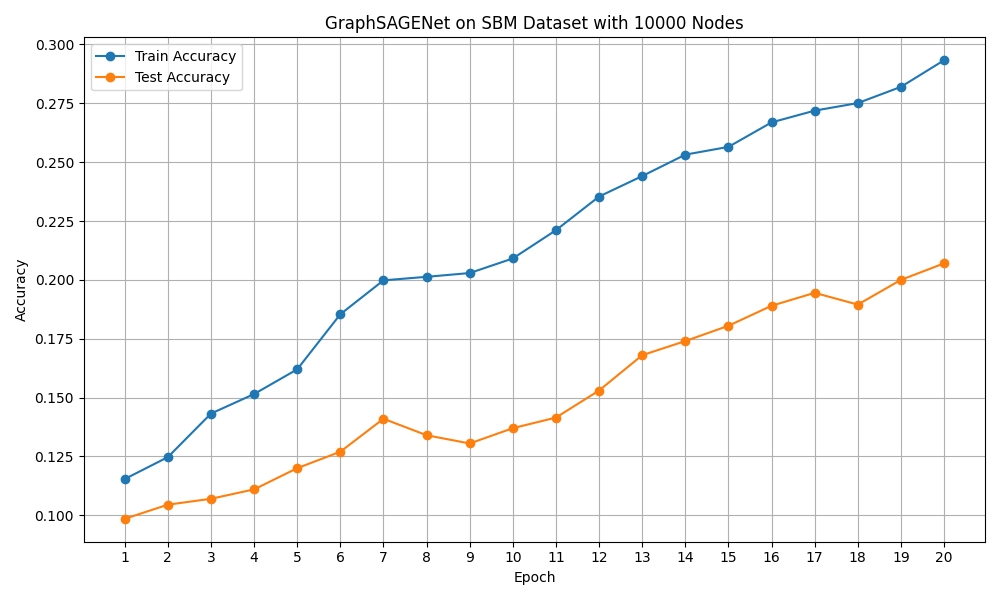
\includegraphics[width=\textwidth]{GraphSAGENet_on_SBM_Dataset_with_10000_Nodes.png}
%         \caption{GraphSAGE on SBM Dataset.}
%         \label{fig:graphsage_sbm_10000}
%     \end{subfigure}

%     % Third row
%     \begin{subfigure}[b]{0.48\textwidth}
%         \centering
%         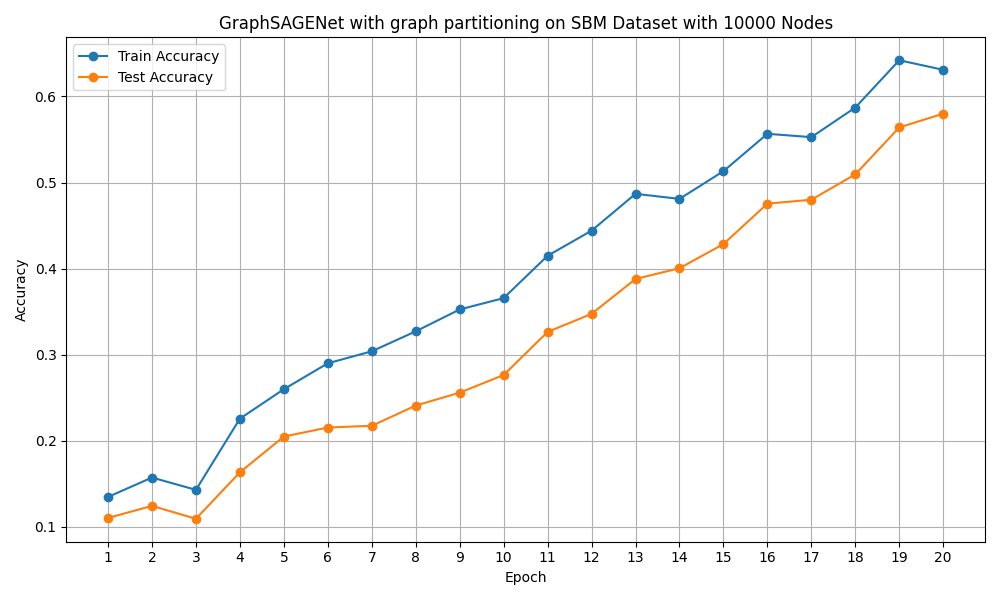
\includegraphics[width=\textwidth]{GraphSAGENet_with_graph_partitioning_on_SBM_Dataset_with_10000_Nodes.png}
%         \caption{GraphSAGE with Graph Partitioning on SBM Dataset.}
%         \label{fig:graphsage_partition_sbm_10000}
%     \end{subfigure}
%     \hfill
%     \begin{subfigure}[b]{0.48\textwidth}
%         \centering
%         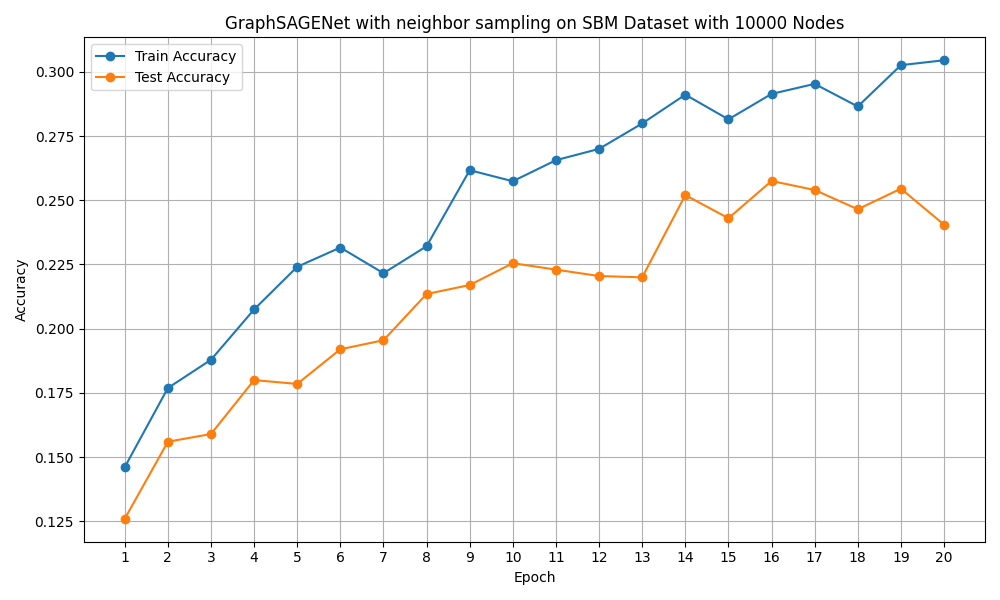
\includegraphics[width=\textwidth]{GraphSAGENet_with_neighbor_sampling_on_SBM_Dataset_with_10000_Nodes.png}
%         \caption{GraphSAGE with Neighbor Sampling on SBM Dataset.}
%         \label{fig:graphsage_neighbor_sbm_10000}
%     \end{subfigure}

%     \caption{Performance comparison on the SBM dataset with 10,000 nodes for GCN and GraphSAGE models under different training strategies: Full-Batch, Graph Partitioning, and Neighbor Sampling.}
%     \label{fig:performance_sbm_10000}
% \end{figure}

\subsubsection{Performance Summary Tables}

% \paragraph{SBM Dataset with 1,000 Nodes}
\begin{table}[H]
    \centering
    \caption{Performance on SBM Dataset with 1,000 Nodes.}
    \label{tab:sbm_1000}
    \begin{tabular}{|l|l|c|c|c|c|}
        \hline
        \textbf{Model} & \textbf{Method} & \textbf{Test Accuracy} & \textbf{Train Time (s)} \\ \hline
        \multirow{3}{*}{GCNet} & Full Batch & 70\% & 0.19 \\ \cline{2-4}
                              & Neighbor Sampling & 67\% & 3.32 \\ \cline{2-4}
                              & Graph Partitioning & 50.5\% & 0.58 \\ \hline
        \multirow{3}{*}{GraphSAGENet} & Full Batch & 52.5\% & 0.13 \\ \cline{2-4}
                                      & Neighbor Sampling & 85.5\% & 3.17 \\ \cline{2-4}
                                      & Graph Partitioning & 46\% & 0.65 \\ \hline
    \end{tabular}
\end{table}

% \paragraph{SBM Dataset with 10,000 Nodes}
\begin{table}[H]
    \centering
    \caption{Performance on SBM Dataset with 10,000 Nodes.}
    \label{tab:sbm_10000}
    \begin{tabular}{|l|l|c|c|c|c|}
        \hline
        \textbf{Model} & \textbf{Method} & \textbf{Test Accuracy} & \textbf{Train Time (s)} \\ \hline
        \multirow{3}{*}{GCNet} & Full Batch & 90\% & 12.66 \\ \cline{2-4}
                              & Neighbor Sampling & 17.85\% & 44.62 \\ \cline{2-4}
                              & Graph Partitioning & 89.85\% & 9.51 \\ \hline
        \multirow{3}{*}{GraphSAGENet} & Full Batch & 20.7\% & 10.23 \\ \cline{2-4}
                                      & Neighbor Sampling & 24.05\% & 42.07 \\ \cline{2-4}
                                      & Graph Partitioning & 58\% & 8.40 \\ \hline
    \end{tabular}
\end{table}

% \paragraph{CORA Dataset}
\begin{table}[H]
    \centering
    \caption{Performance on CORA Dataset.}
    \label{tab:cora}
    \begin{tabular}{|l|l|c|c|c|c|}
        \hline
        \textbf{Model} & \textbf{Method} & \textbf{Test Accuracy} & \textbf{Train Time (s)} \\ \hline
        \multirow{3}{*}{GCNet} & Full Batch & 89.48\% & 0.19 \\ \cline{2-4}
                              & Neighbor Sampling & 88.01\% & 4.86 \\ \cline{2-4}
                              & Graph Partitioning & 87.08\% & 0.86 \\ \hline
        \multirow{3}{*}{GraphSAGENet} & Full Batch & 90.41\% & 0.88 \\ \cline{2-4}
                                      & Neighbor Sampling & 88.56\% & 8.93 \\ \cline{2-4}
                                      & Graph Partitioning & 88.75\% & 1.58 \\ \hline
    \end{tabular}
\end{table}

% \paragraph{Reddit Dataset}
\begin{table}[H]
    \centering
    \caption{Performance on Reddit Dataset.}
    \label{tab:reddit}
    \begin{tabular}{|l|l|c|c|c|c|}
        \hline
        \textbf{Model} & \textbf{Method} & \textbf{Test Accuracy} & \textbf{Train Time (s)} \\ \hline
        \multirow{3}{*}{GCNet} & Full Batch & N/A (Out of Memory) & N/A \\ \cline{2-4}
                              & Neighbor Sampling & 88.6\% & 1892.33 \\ \cline{2-4}
                              & Graph Partitioning & 88.12\% & 1688.57 \\ \hline
        \multirow{3}{*}{GraphSAGENet} & Full Batch & N/A (Out of Memory) & N/A \\ \cline{2-4}
                                      & Neighbor Sampling & 86.44\% & 13108.7 \\ \cline{2-4}
                                      & Graph Partitioning & N/A (Out of Memory) & N/A \\ \hline
    \end{tabular}
\end{table}

% \subsection{Discussion}
% The results demonstrate the effectiveness of scalable GNN training methods. Neighbor Sampling strikes a balance between accuracy and computational efficiency, while Graph Partitioning offers the best memory optimization. These findings validate the proposed approaches for handling large-scale graphs and emphasize the importance of choosing the right method based on the dataset and computational constraints.



\section{Conclusion}
% Summarize the key points of your proposal, restating the problem, motivation, and approach. Mention anticipated outcomes and contributions to machine learning.
% In conclusion, this project looks to overcome the limitations present in traditional community detection approaches by using advanced machine learning methods, specifically Graph Neural Networks (GNNs). Traditional methods, such as modularity-based and optimization methods, often struggle with generalizability and the ability to adapt to networks of varying sizes and structures. By focusing on both accuracy and scalability, this approach is aimed at making community detection more useful for large, complex networks.\\\\ This project not only applies theoretical ideas from the course but also shows how they can be used for real-world challenges in network analysis. Through this work, there's a chance to understand network structures better and how advanced machine learning models help improve community detection. This paper showcases the potential of advanced deep learning models, such as GNNs, to optimize the solutions to the NP-Hard problem of 'Community Detection' in social networks.

In conclusion, this study demonstrates the effectiveness of scalable Graph Neural Network (GNN) training methods for addressing the challenges of community detection in large-scale graphs. Neighbor Sampling offers a balance between accuracy and computational efficiency, while Graph Partitioning provides superior memory optimization, emphasizing the importance of selecting the appropriate method based on dataset characteristics and resource constraints. By leveraging GNNs, this work overcomes the limitations of traditional modularity-based and optimization approaches, which often lack generalizability and scalability. The proposed methodologies enhance the practicality of community detection in large, complex networks, bridging the gap between theoretical advancements and real-world applications. These findings not only contribute to a deeper understanding of network structures but also highlight the potential of advanced deep learning techniques to tackle the NP-hard problem of community detection effectively.

% \section*{References}


\bibliography{ref}
% List references here, providing citations to support the motivation and related work. Ensure consistent citation formatting. Adjust font size if necessary to remain within the 5-page limit.

\end{document}